\documentclass[aspectratio=169,xcolor=dvipsnames]{beamer}

\AtBeginSection[]
{
    \begin{frame}
        \frametitle{Visão Geral}
        \tableofcontents[currentsection]
    \end{frame}
}

\usefonttheme{professionalfonts} % using non standard fonts for beamer
\usefonttheme{serif} % default family is serif
\usepackage{fontspec}
\setmainfont{XCharter}[
    UprightFont    = *-Roman,
    BoldFont       = *-Bold,
    ItalicFont     = *-Italic,
    BoldItalicFont = *-BoldItalic,
]

\usepackage{hyperref}
\usepackage{graphicx} % Allows including images
\usepackage{booktabs} % Allows the use of \toprule, \midrule and \bottomrule in tables
\input{./slides/SimplePlusTheme/beamerthemeSimplePlus.sty}
\input{./slides/SimplePlusTheme/beamerinnerthemeSimplePlus.sty}
\input{./slides/SimplePlusTheme/beamerfontthemeSimplePlus.sty}
\input{./slides/SimplePlusTheme/beamercolorthemeSimplePlus.sty}

\usepackage{listings}
\setbeamercovered{transparent}

\usepackage{biblatex}
\addbibresource{slides/reference.bib}
\renewcommand*{\bibfont}{\footnotesize}

\usepackage[brazilian ]{babel}
\usepackage{csquotes}
\usepackage{pgfplots}
\pgfplotsset{compat=1.18}

\usepackage{emoji}
\usepackage{amsmath}
\usepackage[xcharter,bigdelims,vvarbb]{newtxmath}
% newtxmath's operators font requests the fontspec family `XCharter(0)' in OT1;
% without these substitutions math digits and operator names silently fall back
% to Computer Modern (LaTeX Font Warning: Font shape `OT1/XCharter(0)/m/n' undefined).
\DeclareFontFamily{OT1}{XCharter(0)}{}
\DeclareFontShape{OT1}{XCharter(0)}{m}{n}{<->ssub * XCharter-TLF/m/n}{}
\DeclareFontShape{OT1}{XCharter(0)}{m}{it}{<->ssub * XCharter-TLF/m/it}{}
\DeclareFontShape{OT1}{XCharter(0)}{b}{n}{<->ssub * XCharter-TLF/b/n}{}
\DeclareFontShape{OT1}{XCharter(0)}{bx}{n}{<->ssub * XCharter-TLF/b/n}{}

\usepackage{bm}
\usepackage[table]{xcolor}
\usepackage{xcolor}
\usepackage{algpseudocode}

\usepackage{cancel}
\usepackage{ulem}

\usetikzlibrary{shapes}
\usetikzlibrary{arrows}
\usetikzlibrary {arrows.meta}
\usetikzlibrary{calc,positioning}
\usepgfplotslibrary{fillbetween}
\usetikzlibrary{angles,quotes}
\usetikzlibrary{tikzmark}


\definecolor{PastelRed}{HTML}{FFC1CC}
\definecolor{PastelBlue}{HTML}{C2F0FF}
\definecolor{PastelBlue2}{HTML}{3182BD}

\definecolor{PastelPink}{HTML}{FFCBE1}
\definecolor{PastelGreen}{HTML}{D6E5BD}
\definecolor{PastelYellow}{HTML}{F9E1A8}
\definecolor{PastelBlue}{HTML}{BCD8EC}
\definecolor{PastelPurple}{HTML}{DCCCEC}
\definecolor{PastelOrange}{HTML}{FFDAB4}


\renewcommand{\footnotesize}{\tiny}

\newcommand{\mespor}{
  \ifcase\month
    \or janeiro
    \or fevereiro
    \or março
    \or abril
    \or maio
    \or junho
    \or julho
    \or agosto
    \or setembro
    \or outubro
    \or novembro
    \or dezembro
  \fi
}
% \usepackage{csquotes}
% \usepackage{minted}
% \usemintedstyle{xcode}
\definecolor{vscLightBackground}{HTML}{FFFFFF}
\definecolor{vscLightText}{HTML}{000000}
\definecolor{vscLightGreen}{HTML}{008000}        % For Comments AND Numbers
\definecolor{vscLightRed}{HTML}{A31515}          % For Strings
\definecolor{vscLightTeal}{HTML}{267F99}
\definecolor{vscBlue}{HTML}{0000FF}% For main keywords (if, for, def...)
\definecolor{vscLightPytorch}{HTML}{800080}      % For PyTorch keywords (dark magenta)

\lstdefinestyle{vscode-light}{
    language=Python,
    backgroundcolor=\color{vscLightBackground},
    basicstyle=\ttfamily\scriptsize\color{vscLightText},
    keywordstyle=\color{vscLightTeal},
    commentstyle=\color{vscLightGreen},
    stringstyle=\color{vscLightRed},
    % Style for PyTorch keywords (using keyword group 2)
    keywordstyle=[2]\color{vscLightPytorch}, 
    morekeywords={self, True, False, None},
    morekeywords=[2]{
        torch, Tensor, device, dtype, to, nn, optim, autograd, utils, data,
        Module, Linear, Conv2d, ReLU, CrossEntropyLoss, Adam, SGD,
        Dataset, DataLoader, randn, zeros, ones, arange, cat, stack,
        view, reshape, sum, mean, max, min, matmul, no_grad, backward
    },
    keywordstyle=[3]\color{vscBlue}, 
    morekeywords=[3]{
        model, loss, y, y_hat, x , optimizer
    },
    frame=single,
    tabsize=1,
    showstringspaces=false,
    breaklines=true,
    captionpos=b,
    extendedchars=true,
    numbers=left,
}

\usepackage[cache=true]{minted}
% minted v3+ (TeX Live 2024+) auto-detects the output directory.
% minted v2 (Ubuntu apt TeX Live 2023) needs it set explicitly to
% match latexmkrc's $out_dir = 'build'.
\makeatletter
\@ifpackagelater{minted}{2024/01/01}{}{%
  \def\minted@outputdir{build/}%
}
\makeatother
\setminted{
    fontsize=\scriptsize,
    style=vs,
    breaklines=true,
    numbers=left,
    numbersep=5pt,
    frame=single,
}
\providecommand{\citeauthoryear}[1]{(\citeauthor{#1},~\citeyear{#1})}

\providecommand{\thetav}{\bm{\theta}}

\providecommand{\varvector}[1]{\mathbf{#1}}
% instance
\providecommand{\X}{\varvector{X}}
\providecommand{\mlinstance}{\varvector{X}}
\providecommand{\mlinstancei}{\varvector{X}^{(i)}}
\providecommand{\mlinstancex}[1]{\varvector{X}^{(#1)}}

% target
\providecommand{\y}{\varvector{y}}
\providecommand{\mltarget}{\varvector{y}}
\providecommand{\mltargeti}{\varvector{y}^{(i)}}
\providecommand{\mltargetx}[1]{\varvector{y}^{(#1)}}

%hats
\providecommand{\yhat}{\hat{\varvector{y}}}
\providecommand{\mltargethat}{\hat{\varvector{y}}}
\providecommand{\mltargethati}{\hat{\varvector{y}}^{(i)}}
\providecommand{\mltargethatx}[1]{\hat{\varvector{y}}^{(#1)}}

% linear reg
\providecommand{\mllinearregression}{\mltargethat=\mlinstance\bm{\theta}}

\providecommand{\tikzarrowcolor}[3]{%
  \begin{tikzpicture}[remember picture, overlay]
    % Arrow body
    \path[fill=#3] ([shift={(#1,#2)}]current page.south west) 
      rectangle ++(0.3, -0.2);
    % Arrow head
    \path[fill=#3] ([shift={(#1+0.3,#2+0.1)}]current page.south west) -- 
         ++(0, -0.4) -- 
         ++(0.2, 0.2) -- 
         cycle;
  \end{tikzpicture}%
}

\providecommand{\tikzarrow}[2]{%
    \tikzarrowcolor{#1}{#2}{Red}
}



\DeclareMathOperator*{\argmax}{argmax}
\DeclareMathOperator*{\argmin}{argmin}



% Bibliotecas TikZ adicionais usadas neste deck
\usetikzlibrary{matrix,fit,backgrounds}

% Cores locais para consistência com o material original
\definecolor{qcolor}{RGB}{139,76,177}      % roxo (queries)
\definecolor{kcolor}{RGB}{218,165,32}      % dourado (keys)
\definecolor{vcolor}{RGB}{52,152,219}      % azul (values)
\definecolor{embcolor}{RGB}{120,180,90}    % verde (embeddings)
\definecolor{lightyellow}{RGB}{255,252,220}
\definecolor{lightblue}{RGB}{220,235,252}
\definecolor{lightgreen}{RGB}{220,245,220}
\definecolor{lightred}{RGB}{255,225,225}
\definecolor{lightpurple}{RGB}{230,220,255}
\definecolor{lightorange}{RGB}{255,237,210}
\definecolor{darkgreen}{RGB}{0,120,0}
\definecolor{encblock}{RGB}{215,238,210}
\definecolor{decblock}{RGB}{255,225,210}
% Cores dos blocos da figura da arquitetura
\definecolor{embblock}{RGB}{252,222,222}
\definecolor{mhablock}{RGB}{255,228,185}
\definecolor{ffblock}{RGB}{200,228,250}
\definecolor{normblock}{RGB}{240,240,190}
\definecolor{linblock}{RGB}{215,215,240}
\definecolor{smblock}{RGB}{200,235,205}
\definecolor{stackfill}{RGB}{243,243,243}

% Atalhos para destacar Q, K, V em fórmulas
\newcommand{\Qc}{\textcolor{qcolor}{\mathbf{Q}}}
\newcommand{\Kc}{\textcolor{kcolor}{\mathbf{K}}}
\newcommand{\Vc}{\textcolor{vcolor}{\mathbf{V}}}

% Coluna de três "bolinhas" (vetor) para o diagrama de self-attention.
% #1: nome do nó; #2, #3: coordenadas x, y; #4: cor das bolinhas.
\newcommand{\vecol}[4]{%
    \node[vec] (#1) at (#2, #3) {};
    \foreach \o in {-0.22, 0, 0.22} { \fill[#4] (#2, #3+\o) circle (0.06); }
}

% ------------------------------------------------------------
% Figura da arquitetura encoder-decoder (Vaswani et al., 2017) em TikZ.
% #1: código extra desenhado por cima da figura, tipicamente destaques
%     do tipo \node[foco, fit=(enc-mha)] {};
% Nós nomeados: enc-in, enc-emb, enc-plus, enc-pe, enc-mha, enc-an1, enc-ff,
%   enc-an2, enc-box, dec-in, dec-emb, dec-plus, dec-pe, dec-mmha, dec-an1,
%   dec-xmha, dec-an2, dec-ff, dec-an3, dec-box, out-lin, out-sm, out-prob.
% ------------------------------------------------------------
\tikzset{foco/.style={draw=red, line width=1.4pt, rounded corners=3pt, inner sep=2pt}}
\newcommand{\transformerfig}[1]{%
\begin{tikzpicture}[
    >=Stealth, font=\scriptsize,
    blk/.style={draw, rounded corners=2pt, minimum width=2.2cm, minimum height=0.44cm, align=center, inner sep=2pt},
    emb/.style={blk, fill=embblock},
    mha/.style={blk, fill=mhablock},
    an/.style={blk, fill=normblock, minimum height=0.34cm},
    ff/.style={blk, fill=ffblock},
    lin/.style={blk, fill=linblock, minimum height=0.34cm},
    sm/.style={blk, fill=smblock, minimum height=0.34cm},
    plus/.style={draw, circle, inner sep=0pt, minimum size=0.28cm, fill=white, font=\footnotesize},
    pe/.style={draw, circle, inner sep=0pt, minimum size=0.34cm, fill=white},
    arr/.style={->, thick},
    lbl/.style={font=\tiny, align=center},
]
    % ---------------- Encoder (coluna x = 0) ----------------
    \node[lbl] (enc-in) at (0,0) {Entrada\\(origem)};
    \node[emb, above=0.3cm of enc-in] (enc-emb) {Input\\Embedding};
    \node[plus, above=0.3cm of enc-emb] (enc-plus) {$+$};
    \node[pe, left=0.3cm of enc-plus] (enc-pe) {\scalebox{0.7}{$\sim$}};
    \node[lbl, left=0.05cm of enc-pe] {Positional\\Encoding};
    \node[mha, above=0.75cm of enc-plus] (enc-mha) {Multi-Head\\Attention};
    \node[an, above=0.22cm of enc-mha] (enc-an1) {Add \& Norm};
    \node[ff, above=0.4cm of enc-an1] (enc-ff) {Feed\\Forward};
    \node[an, above=0.22cm of enc-ff] (enc-an2) {Add \& Norm};

    \draw[arr] (enc-in) -- (enc-emb);
    \draw[arr] (enc-emb) -- (enc-plus);
    \draw[arr] (enc-pe) -- (enc-plus);
    \coordinate (enc-split) at ($(enc-plus.north)+(0,0.3)$);
    \draw[thick] (enc-plus.north) -- (enc-split);
    \draw[arr] (enc-split) -- (enc-mha.south);
    \draw[arr] (enc-split) to[out=90,in=-90] ([xshift=-0.65cm]enc-mha.south);
    \draw[arr] (enc-split) to[out=90,in=-90] ([xshift=0.65cm]enc-mha.south);
    \draw[arr] (enc-mha) -- (enc-an1);
    \draw[arr] (enc-an1) -- (enc-ff);
    \draw[arr] (enc-ff) -- (enc-an2);
    % residuais (pela esquerda)
    \draw[arr] (enc-split) -- ++(-1.45,0) |- (enc-an1.west);
    \coordinate (enc-r2) at ($(enc-an1.north)!0.5!(enc-ff.south)$);
    \draw[arr] (enc-r2) -- ++(-1.45,0) |- (enc-an2.west);

    % ---------------- Decoder (coluna x = 4.6) ----------------
    \node[lbl] (dec-in) at (4.6,0) {Saída\\(deslocada à direita)};
    \node[emb, above=0.3cm of dec-in] (dec-emb) {Output\\Embedding};
    \node[plus, above=0.3cm of dec-emb] (dec-plus) {$+$};
    \node[pe, right=0.3cm of dec-plus] (dec-pe) {\scalebox{0.7}{$\sim$}};
    \node[lbl, right=0.05cm of dec-pe] {Positional\\Encoding};
    \node[mha, above=0.75cm of dec-plus, minimum height=0.6cm] (dec-mmha) {Masked\\Multi-Head\\Attention};
    \node[an, above=0.22cm of dec-mmha] (dec-an1) {Add \& Norm};
    \node[mha, above=0.75cm of dec-an1] (dec-xmha) {Multi-Head\\Attention};
    \node[an, above=0.22cm of dec-xmha] (dec-an2) {Add \& Norm};
    \node[ff, above=0.4cm of dec-an2] (dec-ff) {Feed\\Forward};
    \node[an, above=0.22cm of dec-ff] (dec-an3) {Add \& Norm};
    \node[lin, above=0.4cm of dec-an3] (out-lin) {Linear};
    \node[sm, above=0.22cm of out-lin] (out-sm) {Softmax};
    \node[lbl, above=0.25cm of out-sm] (out-prob) {Probabilidades\\do próximo token};

    \draw[arr] (dec-in) -- (dec-emb);
    \draw[arr] (dec-emb) -- (dec-plus);
    \draw[arr] (dec-pe) -- (dec-plus);
    \coordinate (dec-split) at ($(dec-plus.north)+(0,0.3)$);
    \draw[thick] (dec-plus.north) -- (dec-split);
    \draw[arr] (dec-split) -- (dec-mmha.south);
    \draw[arr] (dec-split) to[out=90,in=-90] ([xshift=-0.65cm]dec-mmha.south);
    \draw[arr] (dec-split) to[out=90,in=-90] ([xshift=0.65cm]dec-mmha.south);
    \draw[arr] (dec-mmha) -- (dec-an1);
    % query da cross-attention vem do decoder
    \coordinate (dec-split2) at ($(dec-an1.north)+(0,0.15)$);
    \draw[thick] (dec-an1.north) -- (dec-split2);
    \draw[arr] (dec-split2) to[out=90,in=-90] ([xshift=0.65cm]dec-xmha.south);
    \draw[arr] (dec-xmha) -- (dec-an2);
    \draw[arr] (dec-an2) -- (dec-ff);
    \draw[arr] (dec-ff) -- (dec-an3);
    \draw[arr] (dec-an3) -- (out-lin);
    \draw[arr] (out-lin) -- (out-sm);
    \draw[arr] (out-sm) -- (out-prob);
    % residuais (pela direita)
    \draw[arr] (dec-split) -- ++(1.45,0) |- (dec-an1.east);
    \draw[arr] (dec-split2) -- ++(1.45,0) |- (dec-an2.east);
    \coordinate (dec-r3) at ($(dec-an2.north)!0.5!(dec-ff.south)$);
    \draw[arr] (dec-r3) -- ++(1.45,0) |- (dec-an3.east);

    % keys e values da cross-attention vêm da saída do encoder
    \coordinate (enc-out) at ($(enc-an2.north)+(0,0.35)$);
    \coordinate (kv) at ($(dec-xmha.south)+(-1.6,-0.3)$);
    \coordinate (kv-k) at ($(dec-xmha.south)+(-0.65,-0.3)$);
    \coordinate (kv-v) at ($(dec-xmha.south)+(0,-0.3)$);
    \draw[thick] (enc-an2.north) -- (enc-out) -| (kv) -- (kv-v);
    \draw[arr] (kv-k) -- ([xshift=-0.65cm]dec-xmha.south);
    \draw[arr] (kv-v) -- (dec-xmha.south);

    % caixas das pilhas
    \begin{scope}[on background layer]
        \coordinate (enc-boxL) at ($(enc-mha.west)+(-1.3,0)$);
        \coordinate (dec-boxR) at ($(dec-mmha.east)+(1.3,0)$);
        \node[draw, rounded corners=4pt, fill=stackfill, inner sep=4pt,
              fit=(enc-mha)(enc-an2)(enc-boxL)] (enc-box) {};
        \node[draw, rounded corners=4pt, fill=stackfill, inner sep=4pt,
              fit=(dec-mmha)(dec-an3)(dec-boxR)] (dec-box) {};
    \end{scope}
    \node[lbl, left=0.05cm of enc-box] {$N\times$};
    \node[lbl, right=0.05cm of dec-box] {$N\times$};
    \node[lbl, anchor=south west, text=darkgray] at ([yshift=1pt]enc-box.north west) {Encoder};
    \node[lbl, anchor=south east, text=darkgray] at ([yshift=1pt]dec-box.north east) {Decoder};

    #1
\end{tikzpicture}%
}

% Slide da arquitetura em duas colunas.
% #1 (opcional): título do frame; #2: texto da coluna esquerda;
% #3: destaques desenhados sobre a figura (ex.: \node[foco, fit=(enc-mha)] {};).
\newcommand{\archslide}[3][A Arquitetura Completa]{%
\begin{frame}{#1}
\begin{columns}[c]
\begin{column}{0.46\textwidth}
#2
\end{column}
\begin{column}{0.50\textwidth}
\centering
\resizebox{!}{0.82\textheight}{\transformerfig{#3}}
\end{column}
\end{columns}
\end{frame}
}

\title{Transformers}
\subtitle{Atenção, Self-Attention e a Arquitetura Encoder-Decoder}
\author{Lucas Silveira Kupssinskü}
\institute{Machine Learning Theory and Applications Laboratory \\ PUCRS}
\date{\mespor de \the\year}

\begin{document}

% ============================================================
\begin{frame}
    \titlepage
\end{frame}

% ============================================================
\begin{frame}{Visão Geral}
    \tableofcontents
\end{frame}

% ============================================================
\section{A Tarefa e a Arquitetura}
% ============================================================

\archslide[O Transformer]{
A figura ao lado é a arquitetura proposta em \textit{Attention is All You Need} (Vaswani et al., 2017).

\vspace{6pt}

Ela \textbf{transforma uma sequência em outra}, por exemplo, traduz uma frase.
}{}

% ============================================================

\begin{frame}{A Tarefa: Tradução Automática}

Recebemos uma frase na língua de \textbf{origem} e produzimos a frase correspondente na língua \textbf{alvo}. O conjunto de treino é formado por pares de frases:

\vspace{2pt}

\begin{center}
\renewcommand{\arraystretch}{1.4}
\begin{tabular}{ll}
\toprule
\textbf{Origem (português)} & \textbf{Alvo (inglês)} \\
\midrule
O gato sentou no tapete. & The cat sat on the mat. \\
Eu vi um gato no tapete. & I saw a cat on the mat. \\
Ontem choveu muito em Porto Alegre. & It rained a lot in Porto Alegre yesterday. \\
\bottomrule
\end{tabular}
\end{center}

\vspace{2pt}

\begin{block}{O que a tarefa exige}
\begin{itemize}
    \item Origem e alvo têm \textbf{comprimentos diferentes}, e cada frase tem o seu
    \item A ordem das palavras muda (\textit{ontem} abre a frase em português e fecha em inglês)
    \item Cada palavra do alvo depende de \textbf{toda} a origem e das palavras já escritas
\end{itemize}
\end{block}

\end{frame}

% ============================================================

\begin{frame}[shrink=10]{Gerar a Saída Token a Token}

O modelo produz a frase alvo \textbf{um token por vez}: a cada passo recebe a origem inteira e o que já escreveu, e devolve uma \textbf{distribuição de probabilidade} sobre o vocabulário para o próximo token.

\begin{center}
Origem (fixa em todos os passos): \texttt{O gato sentou no tapete}

\renewcommand{\arraystretch}{1.1}
\begin{tabular}{cll}
\toprule
\textbf{Passo} & \textbf{Já escrito} & \textbf{Próximo token mais provável} \\
\midrule
1 & \texttt{<bos>} & The \\
2 & \texttt{<bos>} The & cat \\
3 & \texttt{<bos>} The cat & sat \\
$\vdots$ & & \\
7 & \texttt{<bos>} The cat sat on the mat & \texttt{<eos>} \\
\bottomrule
\end{tabular}
\end{center}

\begin{itemize}
    \item O token escolhido é \textbf{realimentado} como entrada do passo seguinte; paramos ao gerar \texttt{<eos>}. Esse processo, chamado \textbf{autoregressivo}, vale para qualquer geração de texto
    \item Na figura, o \textbf{encoder} lê a origem e o \textbf{decoder} escreve o alvo
\end{itemize}

\end{frame}

% ============================================================
\section{Tokens e Embeddings}
% ============================================================

\begin{frame}{Da Frase aos Índices}

Redes neurais operam sobre números. O primeiro passo é quebrar o texto em \textbf{tokens} e trocar cada token pelo seu \textbf{índice} em um vocabulário $V$ fixo.

\vspace{8pt}

\begin{center}
\renewcommand{\arraystretch}{1.4}
\begin{tabular}{lcl}
texto & & \texttt{O gato sentou no tapete} \\
tokens & $\rightarrow$ & \texttt{[O] [gato] [sentou] [no] [tapete]} \\
índices & $\rightarrow$ & \texttt{[12, 845, 2210, 7, 3391]} \\
\end{tabular}
\end{center}

\vspace{8pt}

\begin{itemize}
    \item Um token pode ser uma palavra, um pedaço de palavra ou um caractere; o vocabulário é construído por um algoritmo de \textbf{tokenização}, como o BPE
    \item A sequência de $m$ tokens vira um vetor de $m$ inteiros entre $0$ e $|V|-1$
    \item Um índice não carrega significado: $845$ e $846$ podem ser palavras sem relação alguma
\end{itemize}

\end{frame}

% ============================================================

\begin{frame}{Input Embedding: uma Matriz Aprendida}

Cada token da sequência é um \textbf{índice inteiro} do vocabulário $V$. Precisamos de um vetor com significado para cada um.

\vspace{6pt}

\begin{block}{A camada de embedding}
É uma \textbf{matriz de parâmetros aprendidos}
\[
\mathbf{E} \in \mathbb{R}^{|V| \times d},
\]
com uma linha por token do vocabulário: a linha $t$ é o embedding do token de índice $t$. A matriz é treinada por backpropagation como qualquer outro peso da rede.
\end{block}

\vspace{6pt}

\begin{exampleblock}{Ordem de grandeza}
Com $|V| = 50\,000$ e $d = 512$, a camada de embedding tem $|V| \times d = 25{,}6$ milhões de parâmetros.
\end{exampleblock}

\end{frame}

% ============================================================

\begin{frame}{Selecionando o Embedding de um Token}

Como o modelo seleciona o embedding do token de índice $t$? O índice vira um vetor \textbf{one-hot} $\mathbf{u} \in \{0,1\}^{|V|}$, com $1$ apenas na posição $t$, e o produto $\mathbf{u}^{\top} \mathbf{E}$ devolve exatamente a \textbf{linha $t$} de $\mathbf{E}$.

\vspace{4pt}

\begin{exampleblock}{Exemplo com $|V| = 4$ e $d = 3$, token de índice $3$}
\[
\mathbf{u}^{\top} \mathbf{E} =
\begin{bmatrix} 0 & 0 & 1 & 0 \end{bmatrix}
\begin{bmatrix}
0.2 & -1.1 & 0.7 \\
1.5 & 0.3 & -0.4 \\
-0.8 & 0.9 & 2.1 \\
0.6 & -0.5 & 1.3
\end{bmatrix}
=
\begin{bmatrix} -0.8 & 0.9 & 2.1 \end{bmatrix}
= \mathbf{E}_{3,:}
\]
\end{exampleblock}

\vspace{6pt}

Na prática, os frameworks implementam a operação como \textit{lookup}: indexam a linha $t$ diretamente, sem multiplicação de matrizes.

\end{frame}

% ============================================================

\begin{frame}{A Entrada do Modelo é uma Matriz}

Empilhando os embeddings dos $m$ tokens da frase, a entrada vira uma matriz com \textbf{um token por linha}:
\[
\mathbf{X} =
\begin{bmatrix}
\text{---}\; \mathbf{x}_1 \;\text{---} \\
\text{---}\; \mathbf{x}_2 \;\text{---} \\
\vdots \\
\text{---}\; \mathbf{x}_m \;\text{---}
\end{bmatrix}
\in \mathbb{R}^{m \times d},
\qquad \mathbf{x}_t = \mathbf{E}_{\text{índice}(t),:} \in \mathbb{R}^{d}.
\]

\vspace{6pt}

\begin{block}{Convenção usada em toda a aula}
Vetores são \textbf{linhas}. Uma camada linear multiplica pela direita: $\mathbf{x}\,\mathbf{W}$, com $\mathbf{W} \in \mathbb{R}^{d \times d'}$. Aplicada à matriz inteira, $\mathbf{X}\mathbf{W}$ transforma todos os tokens de uma vez.
\end{block}

\vspace{6pt}

\centering
Daqui em diante, \textbf{tudo} que o transformer faz são operações sobre essa matriz.

\end{frame}

% ============================================================
\section{Atenção}
% ============================================================

\begin{frame}{Um Embedding por Token Não Basta}

O embedding de um token é \textbf{a mesma linha de $\mathbf{E}$} em qualquer frase. O significado, porém, depende dos vizinhos.

\vspace{6pt}

\begin{exampleblock}{A mesma linha de $\mathbf{E}$, dois significados}
\centering
\texttt{sentei no \textcolor{red}{banco} da praça} \qquad \texttt{fui ao \textcolor{red}{banco} sacar dinheiro}
\end{exampleblock}

\vspace{4pt}

\begin{exampleblock}{Quem é \texttt{it}?}
\centering
\texttt{"The animal didn't cross the street because \textcolor{red}{it} was tired"}
\end{exampleblock}

\vspace{6pt}

\begin{block}{O que queremos}
Para cada token $t$, um vetor $\mathbf{c}_t$ que represente o token \textbf{no contexto da frase}: construído a partir de $\mathbf{x}_t$ e dos outros $\mathbf{x}_k$, dando mais peso aos tokens relevantes para $t$.
\end{block}

\end{frame}

% ============================================================

\begin{frame}{Por que Não um MLP sobre a Frase Inteira?}

Uma primeira ideia: concatenar os $m$ embeddings em um vetor de tamanho $m \cdot d$ e passar por um MLP, cuja camada de entrada é
\[
[\mathbf{x}_1;\ \mathbf{x}_2;\ \dots;\ \mathbf{x}_m]\;\mathbf{W}_1, \qquad \mathbf{W}_1 \in \mathbb{R}^{(m d) \times h}.
\]

\vspace{2pt}

\begin{alertblock}{Problemas}
\begin{itemize}
    \item $m$ fica \textbf{fixo}: frases de outro comprimento não cabem, e o número de parâmetros \textbf{cresce com} $m$
    \item A palavra na posição 2 e a mesma palavra na posição 5 são multiplicadas por \textbf{pesos diferentes}
\end{itemize}
\end{alertblock}

\vspace{4pt}

\begin{block}{Requisitos para a operação que procuramos}
\begin{itemize}
    \item Funciona para qualquer $m$, com os \textbf{mesmos parâmetros} em todas as posições
    \item O peso que o token $k$ recebe ao construir $\mathbf{c}_t$ depende do \textbf{conteúdo} de $\mathbf{x}_t$ e $\mathbf{x}_k$
\end{itemize}
\end{block}

\end{frame}

% ============================================================

\begin{frame}{A Ideia: Média Ponderada por Similaridade}

Para um vetor de \textbf{consulta} $\mathbf{q}$ (por exemplo, o token que queremos contextualizar) e os vetores $\mathbf{x}_1, \dots, \mathbf{x}_m$ da frase:

\vspace{4pt}

\begin{exampleblock}{Atenção}
\[
\mathbf{c} = \sum_{k=1}^{m} a_k \, \mathbf{x}_k, \qquad a_k \geq 0, \quad \sum_{k=1}^{m} a_k = 1,
\]
com $a_k$ \textbf{grande} quando $\mathbf{x}_k$ é parecido com $\mathbf{q}$ e \textbf{pequeno} caso contrário.
\end{exampleblock}

\vspace{6pt}

\begin{itemize}
    \item Vale para qualquer $m$: é uma soma sobre os tokens que existirem
    \item Os pesos $a_k$ vêm do \textbf{conteúdo} dos vetores, e são recalculados para cada consulta
    \item O resultado $\mathbf{c}$ tem a mesma dimensão $d$ dos vetores de entrada
\end{itemize}

\vspace{6pt}

\centering
Falta definir ``parecido'': precisamos de uma medida de \textbf{similaridade} entre vetores.

\end{frame}

% ============================================================

\begin{frame}{Intuição: atenção como um dicionário ``suave''}

No tipo \textbf{dicionário}, cada \textbf{chave} (\textit{key}) tem um \textbf{valor} (\textit{value}), e uma \textbf{consulta} (\textit{query}) devolve o valor da chave correspondente.

\vspace{6pt}
\begin{columns}[T]
\begin{column}{0.5\textwidth}
\begin{block}{Dicionário comum}
\centering
\texttt{dic = \{1: 10, 2: 50, 3: 100\}}
\begin{itemize}
    \item \texttt{dic[2]} $\rightarrow$ \texttt{50} (chave exata)
    \item \texttt{dic[1.5]} $\rightarrow$ \textcolor{red}{\texttt{KeyError}}
\end{itemize}
\end{block}
\end{column}
\begin{column}{0.5\textwidth}
\onslide<2->{%
\begin{exampleblock}{Dicionário ``suave''}
Não dá erro: devolve uma \textbf{média dos valores ponderada pela proximidade} às chaves.
\begin{center}
\texttt{dic[1.5]} $\rightarrow$ \texttt{30} \quad {\scriptsize $\left(\tfrac{10+50}{2}\right)$}
\end{center}
\end{exampleblock}
}
\end{column}
\end{columns}

\vspace{6pt}
\onslide<2->{%
\begin{block}{É exatamente a atenção}
A \textcolor{qcolor}{\textbf{query}} é comparada a todas as \textcolor{kcolor}{\textbf{keys}}; quanto maior a similaridade (o \textit{score}), mais peso o \textcolor{vcolor}{\textbf{value}} correspondente recebe na média final.
\end{block}
}

\end{frame}

% ============================================================

\begin{frame}[shrink=10]{Atenção: Scores, Pesos e Contexto}

Para a consulta $\mathbf{q}$ e os vetores $\mathbf{x}_1, \dots, \mathbf{x}_m$, todos em $\mathbb{R}^d$:

\begin{block}{Pipeline}
\begin{enumerate}
    \item \textbf{Score} entre a consulta e cada vetor, usando o \textbf{produto escalar} como similaridade (grande quando os vetores apontam na mesma direção):
    \[
        \mathrm{score}(\mathbf{q}, \mathbf{x}_k) = \mathbf{q}^{\top} \mathbf{x}_k = \sum_{i=1}^{d} q_i \, x_{k,i}, \quad k = 1, 2, \dots, m
    \]
    \item \textbf{Pesos da atenção}, convertendo os scores em uma distribuição com a \textbf{softmax}:
    \[
        a_k = \frac{\exp\bigl(\mathrm{score}(\mathbf{q}, \mathbf{x}_k)\bigr)}{\sum_{i=1}^{m} \exp\bigl(\mathrm{score}(\mathbf{q}, \mathbf{x}_i)\bigr)}
    \]
    \item \textbf{Contexto}, a soma ponderada dos vetores:
    $\displaystyle \mathbf{c} = \sum_{k=1}^{m} a_k \, \mathbf{x}_k$
\end{enumerate}
\end{block}

\vspace{2pt}

A softmax garante pesos positivos que somam $1$ e amplifica as diferenças entre os scores.

\end{frame}

% ============================================================

\begin{frame}{Nota Histórica: de Onde Veio a Atenção}

\begin{block}{Bahdanau et al., 2014}
A atenção surgiu em tradução automática, antes do transformer. Os modelos da época (redes recorrentes) liam a origem inteira e a comprimiam em \textbf{um único vetor}, do qual o decoder tinha que escrever a tradução inteira.
\end{block}

\vspace{6pt}

\begin{itemize}
    \item A atenção foi a solução: a cada token gerado, o decoder usa o seu estado como \textbf{query} e faz uma média ponderada dos vetores de \textbf{todos} os tokens da origem
    \item O decoder passa a ``olhar'' para a parte da origem relevante naquele momento, sem depender de um único vetor-resumo
\end{itemize}

\vspace{6pt}

\begin{exampleblock}{O passo seguinte (Vaswani et al., 2017)}
O transformer mantém a atenção e descarta todo o resto: a arquitetura inteira é construída \textbf{só com atenção} e camadas lineares. É o que o título do artigo anuncia.
\end{exampleblock}

\vspace{2pt}
\centering
\footnotesize Bahdanau, D., Cho, K., \& Bengio, Y. (2014). \textit{Neural machine translation by jointly learning to align and translate.}

\end{frame}

% ============================================================

\begin{frame}{Por que ``scaled''?}

Treinar redes com \textit{dot product attention} pode causar \textbf{vanishing gradient} quando as dimensões dos vetores são grandes.

\vspace{6pt}

\begin{block}{Intuição}
Para vetores de dimensão $d$ grande, $\mathbf{q}^{\top} \mathbf{x}_k$ tende a ter magnitudes grandes. A softmax sobre esses scores satura, fazendo com que quase todos os pesos da atenção fiquem próximos de 0 ou de 1, e o gradiente que atravessa a softmax fica próximo de zero.
\end{block}

\vspace{6pt}

\textbf{Vamos quantificar:} suponha $u_i, v_i \sim \mathcal{N}(0, 1)$ i.i.d., componentes de dois vetores $\mathbf{u}, \mathbf{v} \in \mathbb{R}^d$.

\vspace{4pt}
Calcule $\mathbb{E}[\mathbf{u} \cdot \mathbf{v}]$ e $\mathrm{var}[\mathbf{u} \cdot \mathbf{v}]$.

\end{frame}

% ============================================================

\begin{frame}{Esperança e Variância do Produto Escalar}

\begin{columns}[T]
\begin{column}{0.42\textwidth}
\textbf{Esperança:}
\begin{align*}
\mathbb{E}[\mathbf{u} \cdot \mathbf{v}]
&= \mathbb{E}\!\left[\sum_{i=1}^{d} u_i v_i\right] \\
&= \sum_{i=1}^{d} \mathbb{E}[u_i]\,\mathbb{E}[v_i] = 0
\end{align*}
\onslide<2->{%
\vspace{6pt}
{\footnotesize Para $u_i, v_i \sim \mathcal{N}(0, 1)$ i.i.d., $\mathbb{E}[u_i^2] = \mathrm{var}(u_i) = 1$ (pois $\mathbb{E}[u_i] = 0$), o que justifica os dois últimos passos.}

\vspace{6pt}
\textbf{Conclusão:} $\mathrm{var}[\mathbf{u} \cdot \mathbf{v}]$ cresce linearmente com $d$.
}
\end{column}
\begin{column}{0.58\textwidth}
\onslide<2->{%
\textbf{Variância:} por independência,
\begin{align*}
\mathrm{var}[\mathbf{u} \cdot \mathbf{v}]
&= \sum_{i=1}^{d} \mathrm{var}[u_i v_i] \\[2pt]
&= \sum_{i=1}^{d} \Bigl(\mathbb{E}[u_i^2 v_i^2] - \mathbb{E}[u_i v_i]^2\Bigr) \\[2pt]
&= \sum_{i=1}^{d} \mathbb{E}[u_i^2]\,\mathbb{E}[v_i^2] \\[2pt]
&= \sum_{i=1}^{d} \mathrm{var}(u_i)\,\mathrm{var}(v_i) = d
\end{align*}
}
\end{column}
\end{columns}

\end{frame}

% ============================================================

\begin{frame}{Scaled Dot Product Attention}

Para evitar \textit{scores} com magnitude crescente em $d$, normalizamos por $\sqrt{d}$:

\vspace{6pt}

\begin{exampleblock}{Scaled Dot Product Attention}
\[
\mathrm{score}(\mathbf{q}, \mathbf{x}_k) = \frac{\mathbf{q}^{\top} \mathbf{x}_k}{\sqrt{d}}, \quad k = 1, 2, \dots, m
\]
\[
a_k = \frac{\exp(\mathrm{score}(\mathbf{q}, \mathbf{x}_k))}{\sum_{i=1}^{m} \exp(\mathrm{score}(\mathbf{q}, \mathbf{x}_i))}, \qquad
\mathbf{c} = \sum_{k=1}^{m} a_k \, \mathbf{x}_k
\]
\end{exampleblock}

\vspace{6pt}

\begin{itemize}
    \item Escalar por $\sqrt{d}$ mantém a variância dos scores em $1$
    \item A softmax recebe valores com variância controlada e deixa de saturar
    \item É a forma usada no transformer (Vaswani et al., 2017)
\end{itemize}

\end{frame}

% ============================================================

\begin{frame}[shrink=5]{Atenção da Sequência sobre Ela Mesma}

Até aqui a consulta $\mathbf{q}$ era um vetor qualquer. Voltando ao nosso objetivo, contextualizar cada token:

\vspace{4pt}

\begin{block}{\textit{Self-attention}}
Cada token da sequência faz o papel de \textbf{query contra todos os tokens da mesma sequência}, inclusive ele próprio.
\begin{itemize}
    \item O contexto $\mathbf{c}_t$ do token $t$ é a média dos $\mathbf{x}_k$ ponderada pela similaridade com $\mathbf{x}_t$
    \item Repetimos para $t = 1, \dots, m$: a saída é uma nova sequência de $m$ vetores, cada um \textbf{contextualizado}
\end{itemize}
\end{block}

\begin{exampleblock}{Por exemplo, considere a frase}
\centering
\texttt{"The animal didn't cross the street because \textcolor{red}{it} was tired"}
\end{exampleblock}

Com \texttt{it} como query, esperamos peso alto em \texttt{animal}: o contexto de \texttt{it} passa a carregar a informação de a quem ele se refere.

\vspace{2pt}
\centering
\footnotesize Vaswani, A., Shazeer, N., Parmar, N., Uszkoreit, J., Jones, L., Gomez, A. N., Kaiser, {\L}., \& Polosukhin, I. (2017). Attention is All You Need. \textit{Advances in Neural Information Processing Systems}, v.\ 30.

\end{frame}

% ============================================================

\begin{frame}{Self-Attention: a Forma ``Crua'' Não Funciona}

Aplicar dot product attention diretamente sobre os tokens da entrada $\mathbf{x}_1, \dots, \mathbf{x}_m$:

\vspace{4pt}

\[
\mathrm{score}(\mathbf{x}_t, \mathbf{x}_k) = \frac{\mathbf{x}_t \, \mathbf{x}_k^{\top}}{\sqrt{d}}, \qquad
a_k^{(t)} = \mathrm{softmax}_k\bigl(\mathrm{score}(\mathbf{x}_t, \mathbf{x}_k)\bigr)
\]
\[
\mathbf{c}^{(t)} = \sum_{k=1}^{m} a_k^{(t)} \, \mathbf{x}_k
\]

\vspace{6pt}

\begin{alertblock}{Problema}
Não há \textbf{nada para aprender} aqui: o cálculo é determinístico nas entradas. Sem parâmetros treináveis, \textit{backpropagation} não tem o que ajustar.
\end{alertblock}

\vspace{6pt}

\textbf{Solução:} introduzir três projeções lineares aprendidas para cada token, gerando \textbf{queries}, \textbf{keys} e \textbf{values}.

\end{frame}

% ============================================================

\begin{frame}[shrink=10]{Queries, Keys e Values}

Para cada token $\mathbf{x}_t \in \mathbb{R}^{d_{\text{emb}}}$, projetamos em três vetores via matrizes aprendidas:

\vspace{6pt}

\begin{columns}[T]
\begin{column}{0.52\textwidth}
\begin{flalign*}
\textcolor{qcolor}{\mathbf{q}_t} &= \mathbf{x}_t \, \mathbf{W}_q + \mathbf{b}_q, & \mathbf{W}_q &\in \mathbb{R}^{d_{\text{emb}} \times d}, & \mathbf{q}_t &\in \mathbb{R}^{d} && \\
\textcolor{kcolor}{\mathbf{k}_t} &= \mathbf{x}_t \, \mathbf{W}_k + \mathbf{b}_k, & \mathbf{W}_k &\in \mathbb{R}^{d_{\text{emb}} \times d}, & \mathbf{k}_t &\in \mathbb{R}^{d} && \\
\textcolor{vcolor}{\mathbf{v}_t} &= \mathbf{x}_t \, \mathbf{W}_v + \mathbf{b}_v, & \mathbf{W}_v &\in \mathbb{R}^{d_{\text{emb}} \times d_v}, & \mathbf{v}_t &\in \mathbb{R}^{d_v} &&
\end{flalign*}
\end{column}
\begin{column}{0.48\textwidth}
\textbf{Analogia (recuperação de informação):}
\begin{itemize}
    \item \textcolor{qcolor}{\textbf{Query}}: vetor que codifica uma consulta
    \item \textcolor{kcolor}{\textbf{Key}}: chaves de busca, comparadas às queries
    \item \textcolor{vcolor}{\textbf{Value}}: valor retornado quando query e key são similares
\end{itemize}
\end{column}
\end{columns}

\vspace{6pt}

A atenção passa a ser:
\[
\mathrm{score}(\mathbf{q}_t, \mathbf{k}_i) = \frac{\mathbf{q}_t \, \mathbf{k}_i^{\top}}{\sqrt{d}}, \qquad
a_i^{(t)} = \mathrm{softmax}_i(\mathrm{score}(\mathbf{q}_t, \mathbf{k}_i))
\]
\[
\mathbf{c}^{(t)} = \sum_{i=1}^{m} a_i^{(t)} \, \mathbf{v}_i
\]

\textbf{Agora há parâmetros aprendidos:} $\mathbf{W}_q, \mathbf{W}_k, \mathbf{W}_v$.

\end{frame}

% ============================================================

\begin{frame}{Self-Attention: Diagrama do Cálculo}

\begin{center}
\resizebox{!}{0.66\textheight}{%
\begin{tikzpicture}[
    >=Stealth, font=\small,
    vec/.style={draw=black!55, rounded corners=2pt, minimum width=0.3cm, minimum height=0.82cm, inner sep=0, fill=white},
    score/.style={circle, draw=kcolor!80!black, fill=white, inner sep=0, minimum size=0.17cm},
    rowlbl/.style={font=\footnotesize, text=darkgray, anchor=east, align=right},
]
    \def\dx{1.3}

    % --- rótulos das linhas (nossa notação) ---
    \node[rowlbl] at (-0.95, 0)    {tokens};
    \node[rowlbl] at (-0.95, 0.9) {embeddings $\mathbf{x}_i$};
    \node[rowlbl] at (-0.95, 2.2) {projeções\\\textcolor{kcolor!70!black}{$\mathbf{k}_i$}, \textcolor{vcolor!80!black}{$\mathbf{v}_i$} e \textcolor{qcolor}{$\mathbf{q}_t$}};
    \node[rowlbl] at (-0.95, 3.1) {scores\\$\textcolor{qcolor}{\mathbf{q}_t}\,\textcolor{kcolor!70!black}{\mathbf{k}_i^{\top}}/\sqrt{d}$};
    \node[rowlbl] at (-0.95, 4.55) {pesos $a^{(t)}_i$};
    \node[rowlbl] at (-0.95, 5.45) {contexto\\$\mathbf{c}^{(t)} = \sum_i a^{(t)}_i \textcolor{vcolor!80!black}{\mathbf{v}_i}$};

    % --- tokens, embeddings e projeções k, v ---
    \foreach \i/\w/\col in {1/The/black, 2/animal/black, 3/didn't/black, 4/cross/black, 5/the/black,
                            6/street/black, 7/because/black, 8/it/qcolor, 9/was/black, 10/tired/black} {
        \pgfmathsetmacro{\x}{\dx*(\i-1)}
        \pgfmathsetmacro{\off}{ifthenelse(\i==8, 0.36, 0.21)}
        \node[font=\small\bfseries, text=\col, anchor=base] at (\x, 0) {\w};
        \vecol{e\i}{\x}{0.9}{embcolor}
        \vecol{k\i}{\x-\off}{2.2}{kcolor}
        \vecol{v\i}{\x+\off}{2.2}{vcolor}
        \draw[->, kcolor!80!black] (e\i.north) -- (k\i.south);
        \draw[->, vcolor] (e\i.north) -- (v\i.south);
    }

    % --- query: só o token "it" ---
    \vecol{q}{\dx*7}{2.2}{qcolor}
    \draw[->, qcolor] (e8.north) -- (q.south);

    % --- scores: q_t contra cada k_i ---
    \foreach \i in {1,...,10} {
        \pgfmathsetmacro{\x}{\dx*(\i-1)}
        \node[score] (sc\i) at (\x, 3.1) {};
        \draw[->, qcolor, thin] (q.north) -- (sc\i);
        \draw[->, kcolor!80!black] (k\i.north) -- (sc\i);
        \draw[kcolor!70!black, thin] (sc\i.north) -- (\x, 4.3);
    }

    % --- caixa da softmax: desenhada por cima das linhas dos scores (que passam por ela)
    %     e por baixo das setas dos values (que não passam)
    \node[draw=black!40, fill=black!8, fill opacity=0.6, text opacity=1, minimum width=12.6cm, minimum height=0.46cm, font=\footnotesize] at (5.85, 3.72) {softmax};

    % --- vetor de contexto (saída para "it") ---
    \vecol{c}{\dx*7}{5.45}{orange!85!black}

    % --- pesos (barras) e soma ponderada dos values ---
    \draw[kcolor!80!black] (-0.45, 4.3) -- (12.15, 4.3);
    \foreach \i/\a in {1/0.02, 2/0.55, 3/0.03, 4/0.03, 5/0.02, 6/0.06, 7/0.03, 8/0.12, 9/0.04, 10/0.10} {
        \pgfmathsetmacro{\x}{\dx*(\i-1)}
        \pgfmathsetmacro{\h}{1.5*\a}
        \pgfmathsetmacro{\off}{ifthenelse(\i==8, 0.36, 0.21)}
        \fill[kcolor!45, draw=kcolor!80!black] (\x-0.2, 4.3) rectangle (\x+0.2, 4.3+\h);
        \draw[->, vcolor] (v\i.north) -- (\x+\off+0.05, 4.28);
        \draw[black!60, densely dotted] (\x, 4.3+\h) -- (c.south);
    }

    % --- moldura do self-attention ---
    \node[draw=black!50, dashed, rounded corners=3pt, inner sep=8pt, fit=(k1) (v10) (c)] (sabox) {};
    \node[anchor=north east, font=\footnotesize, text=darkgray] at ([xshift=-3pt, yshift=-2pt]sabox.north east) {self-attention};
\end{tikzpicture}%
}
\end{center}

\centering Com \textbf{it} como query, o maior peso cai em \textbf{animal}: o contexto de \textit{it} absorve o referente.

\end{frame}

% ============================================================

\begin{frame}[shrink=10]{Self-Attention: Exemplo Numérico (Setup)}

\textbf{Embeddings de entrada} (dois tokens, $d_{\text{emb}}=3$):
\[
\mathbf{x}_1 = [1,\ -3,\ 2], \qquad \mathbf{x}_2 = [2,\ -1,\ 1]
\]

\textbf{Matrizes de pesos} (todas com bias $0$, projeção para $d=2$):
\[
\mathbf{W}_q = \begin{bmatrix} 1 & 0 \\ 1 & -1 \\ 0 & -2 \end{bmatrix}, \quad
\mathbf{W}_k = \begin{bmatrix} 1 & 1 \\ 0 & -1 \\ 0 & 0 \end{bmatrix}, \quad
\mathbf{W}_v = \begin{bmatrix} -2 & 1 \\ 0 & 1 \\ 0 & 2 \end{bmatrix}
\]

\vspace{4pt}
\centering
Projetamos cada token aplicando $\mathbf{W}_q, \mathbf{W}_k, \mathbf{W}_v$; os cálculos completos vêm a seguir.

\end{frame}

% ============================================================

\begin{frame}[shrink=10]{Self-Attention: Cálculo das Projeções (\textcolor{qcolor}{Queries})}

Cada token é um vetor linha, multiplicado pela matriz $\mathbf{W}_q$ ($\mathbf{q}_i = \mathbf{x}_i \mathbf{W}_q$):

\begin{align*}
\textcolor{qcolor}{\mathbf{q}_1} = \mathbf{x}_1 \mathbf{W}_q &=
\begin{bmatrix} 1 & -3 & 2 \end{bmatrix}
\begin{bmatrix} 1 & 0 \\ 1 & -1 \\ 0 & -2 \end{bmatrix}
= \begin{bmatrix} 1(1){+}(-3)(1){+}2(0) & \;\; 1(0){+}(-3)(-1){+}2(-2) \end{bmatrix} \\[2pt]
&= \begin{bmatrix} -2 & -1 \end{bmatrix}
\end{align*}

\vspace{4pt}

\begin{align*}
\textcolor{qcolor}{\mathbf{q}_2} = \mathbf{x}_2 \mathbf{W}_q &=
\begin{bmatrix} 2 & -1 & 1 \end{bmatrix}
\begin{bmatrix} 1 & 0 \\ 1 & -1 \\ 0 & -2 \end{bmatrix}
= \begin{bmatrix} 2(1){+}(-1)(1){+}1(0) & \;\; 2(0){+}(-1)(-1){+}1(-2) \end{bmatrix} \\[2pt]
&= \begin{bmatrix} 1 & -1 \end{bmatrix}
\end{align*}

\end{frame}

% ============================================================

\begin{frame}[shrink=10]{Self-Attention: Cálculo das Projeções (\textcolor{kcolor}{Keys})}

O mesmo procedimento com a matriz $\mathbf{W}_k$ ($\mathbf{k}_i = \mathbf{x}_i \mathbf{W}_k$):

\begin{align*}
\textcolor{kcolor}{\mathbf{k}_1} = \mathbf{x}_1 \mathbf{W}_k &=
\begin{bmatrix} 1 & -3 & 2 \end{bmatrix}
\begin{bmatrix} 1 & 1 \\ 0 & -1 \\ 0 & 0 \end{bmatrix}
= \begin{bmatrix} 1(1){+}(-3)(0){+}2(0) & \;\; 1(1){+}(-3)(-1){+}2(0) \end{bmatrix} \\[2pt]
&= \begin{bmatrix} 1 & 4 \end{bmatrix}
\end{align*}

\vspace{4pt}

\begin{align*}
\textcolor{kcolor}{\mathbf{k}_2} = \mathbf{x}_2 \mathbf{W}_k &=
\begin{bmatrix} 2 & -1 & 1 \end{bmatrix}
\begin{bmatrix} 1 & 1 \\ 0 & -1 \\ 0 & 0 \end{bmatrix}
= \begin{bmatrix} 2(1){+}(-1)(0){+}1(0) & \;\; 2(1){+}(-1)(-1){+}1(0) \end{bmatrix} \\[2pt]
&= \begin{bmatrix} 2 & 3 \end{bmatrix}
\end{align*}

\end{frame}

% ============================================================

\begin{frame}[shrink=10]{Self-Attention: Cálculo das Projeções (\textcolor{vcolor}{Values})}

E, por fim, com a matriz $\mathbf{W}_v$ ($\mathbf{v}_i = \mathbf{x}_i \mathbf{W}_v$):

\begin{align*}
\textcolor{vcolor}{\mathbf{v}_1} = \mathbf{x}_1 \mathbf{W}_v &=
\begin{bmatrix} 1 & -3 & 2 \end{bmatrix}
\begin{bmatrix} -2 & 1 \\ 0 & 1 \\ 0 & 2 \end{bmatrix}
= \begin{bmatrix} 1(-2){+}(-3)(0){+}2(0) & \;\; 1(1){+}(-3)(1){+}2(2) \end{bmatrix} \\[2pt]
&= \begin{bmatrix} -2 & 2 \end{bmatrix}
\end{align*}

\vspace{4pt}

\begin{align*}
\textcolor{vcolor}{\mathbf{v}_2} = \mathbf{x}_2 \mathbf{W}_v &=
\begin{bmatrix} 2 & -1 & 1 \end{bmatrix}
\begin{bmatrix} -2 & 1 \\ 0 & 1 \\ 0 & 2 \end{bmatrix}
= \begin{bmatrix} 2(-2){+}(-1)(0){+}1(0) & \;\; 2(1){+}(-1)(1){+}1(2) \end{bmatrix} \\[2pt]
&= \begin{bmatrix} -4 & 3 \end{bmatrix}
\end{align*}

\end{frame}

% ============================================================

\begin{frame}[shrink=15]{Self-Attention: Exemplo Numérico (Cálculo)}

\textbf{Foco no token 1:} usamos $\textcolor{qcolor}{\mathbf{q}_1 = [-2, -1]}$ contra todas as keys.

\vspace{6pt}

\textbf{Scores não normalizados} (vetor linha vezes coluna):
\[
\mathbf{q}_1 \mathbf{k}_1^{\top} =
\begin{bmatrix} -2 & -1 \end{bmatrix}
\begin{bmatrix} 1 \\ 4 \end{bmatrix}
= -6, \qquad
\mathbf{q}_1 \mathbf{k}_2^{\top} =
\begin{bmatrix} -2 & -1 \end{bmatrix}
\begin{bmatrix} 2 \\ 3 \end{bmatrix}
= -7
\]

\vspace{4pt}

\textbf{Normalização por $\sqrt{d}$ (com $d=2$):}
\[
-6 / \sqrt{2} \approx -4.24, \qquad -7 / \sqrt{2} \approx -4.95
\]

\vspace{4pt}

\textbf{Softmax sobre os scores normalizados:}
\[
a_1^{(1)} \approx 0.67, \qquad a_2^{(1)} \approx 0.33
\]

\vspace{4pt}

\textbf{Soma ponderada dos values:}
\[
\mathbf{c}^{(1)} = 0.67 \cdot [-2, 2] + 0.33 \cdot [-4, 3] \approx [-2.66,\ 2.33]
\]

\vspace{4pt}
\centering
O token 1 atende \textbf{principalmente} a si mesmo (0.67), mas incorpora uma fração do token 2 (0.33): a saída é uma média ponderada.

\end{frame}

% ============================================================

\begin{frame}{Forma Matricial: Processar Toda a Sequência de uma Vez}

A implementação anterior processa cada query \textbf{de forma independente}. Como o resultado de cada query não depende das demais (no mesmo passo), podemos vetorizar tudo:

\vspace{4pt}

\begin{exampleblock}{Scaled Dot Product Attention (forma matricial)}
\[
\boxed{\;
\mathrm{attention}(\Qc, \Kc, \Vc) = \mathrm{softmax}\!\left(\frac{\Qc \, \Kc^{\top}}{\sqrt{d}}\right) \Vc
\;}
\]
\end{exampleblock}

\vspace{6pt}

\textbf{Com} ($\mathbf{X}$: \texttt{seq\_size $\times$ emb\_size}):
\begin{itemize}
    \item $\Qc = \mathbf{X} \mathbf{W}_q$, $\quad$ $\mathbf{W}_q$: \texttt{emb\_size $\times$ d}, $\quad$ $\Qc$: \texttt{seq\_size $\times$ d}
    \item $\Kc = \mathbf{X} \mathbf{W}_k$, $\quad$ $\mathbf{W}_k$: \texttt{emb\_size $\times$ d}, $\quad$ $\Kc$: \texttt{seq\_size $\times$ d}
    \item $\Vc = \mathbf{X} \mathbf{W}_v$, $\quad$ $\mathbf{W}_v$: \texttt{emb\_size $\times$ value\_size}, $\quad$ $\Vc$: \texttt{seq\_size $\times$ value\_size}
\end{itemize}

\vspace{4pt}

A matriz $\mathrm{softmax}(\Qc \Kc^{\top} / \sqrt{d})$ tem shape \texttt{seq\_size $\times$ seq\_size}: contém os \textbf{pesos da atenção} de cada token sobre cada token.

\end{frame}

% ============================================================

\begin{frame}[shrink=10]{Forma Matricial: Projeções $\Qc, \Kc, \Vc$}

Empilhando os dois embeddings nas linhas de $\mathbf{X}$ ($2\times3$) e projetando com $\mathbf{W}_q, \mathbf{W}_k, \mathbf{W}_v$ ($3\times2$), cada projeção fica $2\times2$:

\vspace{2pt}
\[
\Qc = \mathbf{X} \mathbf{W}_q =
\begin{bmatrix} 1 & -3 & 2 \\ 2 & -1 & 1 \end{bmatrix}
\begin{bmatrix} 1 & 0 \\ 1 & -1 \\ 0 & -2 \end{bmatrix}
= \begin{bmatrix} -2 & -1 \\ 1 & -1 \end{bmatrix}
\]
\[
\Kc = \mathbf{X} \mathbf{W}_k =
\begin{bmatrix} 1 & -3 & 2 \\ 2 & -1 & 1 \end{bmatrix}
\begin{bmatrix} 1 & 1 \\ 0 & -1 \\ 0 & 0 \end{bmatrix}
= \begin{bmatrix} 1 & 4 \\ 2 & 3 \end{bmatrix}
\]
\[
\Vc = \mathbf{X} \mathbf{W}_v =
\begin{bmatrix} 1 & -3 & 2 \\ 2 & -1 & 1 \end{bmatrix}
\begin{bmatrix} -2 & 1 \\ 0 & 1 \\ 0 & 2 \end{bmatrix}
= \begin{bmatrix} -2 & 2 \\ -4 & 3 \end{bmatrix}
\]

\vspace{2pt}
\centering
Cada \textbf{linha} de $\Qc, \Kc, \Vc$ é o vetor projetado de um token.

\end{frame}

% ============================================================

\begin{frame}[shrink=10]{Forma Matricial: Pipeline Completo}

Com as projeções $\Qc$, $\Kc$ e $\Vc$ já calculadas:
\[
\Qc = \begin{bmatrix} -2 & -1 \\ 1 & -1 \end{bmatrix}, \quad
\Kc = \begin{bmatrix} 1 & 4 \\ 2 & 3 \end{bmatrix}, \quad
\Vc = \begin{bmatrix} -2 & 2 \\ -4 & 3 \end{bmatrix}
\]

\vspace{6pt}

\textbf{Scores e normalização:}
\[
\Qc \, \Kc^{\top} = \begin{bmatrix} -6 & -7 \\ -3 & -1 \end{bmatrix}, \qquad
\frac{\Qc \, \Kc^{\top}}{\sqrt{2}} \approx \begin{bmatrix} -4.24 & -4.95 \\ -2.12 & -0.71 \end{bmatrix}
\]

\vspace{4pt}

\textbf{Softmax (por linha):}
\[
\mathrm{softmax} \approx \begin{bmatrix} 0.67 & 0.33 \\ 0.20 & 0.80 \end{bmatrix}
\]

\vspace{4pt}

\textbf{Saída final:}
\[
\mathrm{attention}(\Qc, \Kc, \Vc) \approx \begin{bmatrix} -2.66 & 2.33 \\ -3.61 & 2.80 \end{bmatrix}
\]

\end{frame}

% ============================================================

\begin{frame}[shrink=5]{Propriedades da Self-Attention}

\begin{block}{É não linear?}
\textbf{Sim:} $\Qc \Kc^{\top} \Vc$ é polinomial de grau 3 nos parâmetros; a softmax já é não-linear.
\end{block}

\begin{columns}[T]
\column{0.48\textwidth}
\begin{block}{Parâmetros independentes do comprimento}
$\mathbf{W}_q, \mathbf{W}_k, \mathbf{W}_v$ têm tamanho fixo e atendem sequências de qualquer comprimento. Cada token é processado pelos \textbf{mesmos pesos}, em qualquer posição.
\end{block}

\column{0.48\textwidth}
\begin{block}{Tudo é matricial}
\begin{itemize}
    \item Toda a sequência é processada de uma vez: fácil de \textbf{paralelizar}
    \item Qualquer par de tokens interage \textbf{diretamente}, em uma única operação, por mais distantes que estejam na frase
\end{itemize}
\end{block}
\end{columns}

\begin{exampleblock}{Bônus: explicabilidade}
Os pesos da atenção formam uma matriz interpretável: dá para plotar e ver quais tokens a rede ``olha''.
\end{exampleblock}

\end{frame}

% ============================================================

\begin{frame}[shrink=10]{O Calcanhar de Aquiles: Falta Informação Posicional}

\begin{alertblock}{Problema}
Da forma como definimos, \textit{self-attention} \textbf{não tem informação sobre a posição} dos tokens na sequência.
\end{alertblock}

\vspace{6pt}

A operação é \textbf{equivariante a permutações}: trocar a ordem das linhas de $\mathbf{X}$ apenas troca, da mesma forma, a ordem das linhas da saída. Nenhum peso de atenção muda, porque os scores dependem só do conteúdo dos tokens.

\vspace{8pt}

\begin{exampleblock}{Consequência}
\centering
\texttt{"lucas comeu pastel no jantar"} $=$ \texttt{"jantar comeu pastel no lucas"}

\vspace{4pt}

Para o modelo, ambas as frases produzem o mesmo conjunto de pesos da atenção.
\end{exampleblock}

\vspace{6pt}

\centering
Precisamos adaptar os embeddings para que carreguem informação sobre a \textbf{posição do token} na sequência.

\end{frame}

% ============================================================
\section{Positional Encoding}
% ============================================================

\begin{frame}{Ideia Geral do Positional Encoding}

\textbf{Ideia:} criar uma codificação para a posição e \textbf{somá-la} ao embedding do token.

\vspace{8pt}

\begin{center}
\begin{tikzpicture}[
    >=Stealth, font=\small,
    box/.style={draw, minimum width=1.6cm, minimum height=1.0cm},
]
    \node[box, fill=lightpurple] (we) at (0, 0) {word emb.};
    \node[font=\Large] at (2.0, 0) {$+$};
    \node[box, fill=lightyellow] (pe) at (4.0, 0) {position emb.};
    \node[font=\Large] at (6.0, 0) {$=$};
    \node[box, fill=lightred] (out) at (8.4, 0) {input do transformer};

    \node[font=\scriptsize, anchor=north] at (we.south) {tamanho $d$};
    \node[font=\scriptsize, anchor=north] at (pe.south) {tamanho $d$};
    \node[font=\scriptsize, anchor=north] at (out.south) {tamanho $d$};
\end{tikzpicture}
\end{center}

\vspace{6pt}

\begin{itemize}
    \item Existem várias formas de definir/aprender embeddings posicionais
    \item No paper original, Vaswani et al.\ (2017) observaram que \textbf{embeddings posicionais aprendidos não melhoraram} resultados em relação a embeddings posicionais \textbf{fixos} (sinusoidal)
\end{itemize}

\end{frame}

% ============================================================

\begin{frame}{Propriedades Desejadas}

Precisamos de uma matriz de posições que codifique adequadamente posições \textbf{absolutas} e \textbf{relativas} dos tokens em uma sequência.

\vspace{8pt}

\begin{block}{Requisitos}
\begin{itemize}
    \item \textbf{Único por posição:} cada posição da sequência tem uma codificação distinta
    \item \textbf{Distâncias relativas consistentes:} o deslocamento entre duas posições é codificado de forma consistente, independentemente do tamanho da sequência
    \item \textbf{Generaliza para qualquer tamanho:} a codificação tem limite superior e inferior bem definidos
    \item \textbf{Determinística:} sem aleatoriedade na inferência
\end{itemize}
\end{block}

\end{frame}

% ============================================================

\begin{frame}{Ideia 1: Usar o Índice da Posição}

\textbf{Proposta:} codificar a posição $i$ pelo próprio número $i$ (ou $i / N$).

\vspace{6pt}

\begin{alertblock}{Problemas}
\begin{itemize}
    \item Sem limite superior bem definido (para sequências arbitrárias)
    \item Os valores ficam grandes para sequências longas, dominando o embedding do token
    \item Normalizar por $N$ resolve o limite, mas a mesma posição relativa passa a depender do tamanho da sequência
\end{itemize}
\end{alertblock}

\vspace{6pt}

\centering
Não funciona.

\end{frame}

% ============================================================

\begin{frame}{Ideia 2: Usar Números Binários}

\textbf{Proposta:} usar a representação binária da posição em $\lceil \log_2 N \rceil$ bits.

\vspace{4pt}

\begin{columns}[T]
\column{0.55\textwidth}
\begin{itemize}
    \item Os bits binários têm \textbf{comportamento periódico}
    \item Bits menos significativos alternam rápido (período 2), mais significativos alternam devagar
    \item Isso é desejável para codificar posições
\end{itemize}

\vspace{6pt}

\begin{alertblock}{Problema}
Redes neurais usam matemática \textbf{contínua}. Interpolar entre representações binárias não preserva a noção de distância. Também não funciona.
\end{alertblock}

\column{0.40\textwidth}
\centering
\footnotesize
\renewcommand{\arraystretch}{1.0}
\begin{tabular}{r|cccc}
$0$ & 0 & 0 & 0 & 0 \\
$1$ & 0 & 0 & 0 & 1 \\
$2$ & 0 & 0 & 1 & 0 \\
$3$ & 0 & 0 & 1 & 1 \\
$4$ & 0 & 1 & 0 & 0 \\
$5$ & 0 & 1 & 0 & 1 \\
$6$ & 0 & 1 & 1 & 0 \\
$7$ & 0 & 1 & 1 & 1 \\
$8$ & 1 & 0 & 0 & 0 \\
$\vdots$ &  &  &  &  \\
$15$ & 1 & 1 & 1 & 1 \\
\end{tabular}
\end{columns}

\end{frame}

% ============================================================

\begin{frame}{Ideia 3: Senos e Cossenos de Frequências Variadas}

\textbf{Proposta:} usar uma combinação de senos e cossenos de diferentes frequências para indicar a posição.

\vspace{2pt}

\begin{block}{Por que funciona}
\begin{itemize}
    \item \textbf{Limite máximo e mínimo bem definidos:} $\sin, \cos \in [-1, 1]$
    \item \textbf{Periodicidade multiescala:} cada dimensão tem sua própria frequência, gerando códigos únicos
    \item \textbf{Linearidade da rotação:} a posição (ângulo) pode ser modificada por uma transformação linear
\end{itemize}
\end{block}

\vspace{2pt}

\[
\begin{pmatrix} \cos(\theta + \phi) \\ \sin(\theta + \phi) \end{pmatrix}
=
\begin{pmatrix} \cos\phi & -\sin\phi \\ \sin\phi & \cos\phi \end{pmatrix}
\begin{pmatrix} \cos\theta \\ \sin\theta \end{pmatrix}
\]

\vspace{2pt}

Isso significa que o modelo consegue ``rotacionar'' as posições por uma matriz de pesos aprendida, capturando deslocamentos relativos.

\end{frame}

% ============================================================

\begin{frame}{Positional Encoding Sinusoidal: Fórmula}

\begin{exampleblock}{Definição (Vaswani et al., 2017)}
\[
P_{i,j} =
\begin{cases}
\sin\!\left(\dfrac{i}{n^{(2k/d)}}\right), & \text{se } j = 2k \\[12pt]
\cos\!\left(\dfrac{i}{n^{(2k/d)}}\right), & \text{se } j = 2k + 1
\end{cases}
\]
\end{exampleblock}

\vspace{4pt}

\textbf{Onde:}
\begin{itemize}
    \item $i$: índice da posição na sequência
    \item $j$: índice da dimensão do embedding ($j = 0, \dots, d-1$)
    \item $d$: dimensão do embedding
    \item $n$: hiperparâmetro de escala (no paper, $n = 10000$)
\end{itemize}

\vspace{4pt}

Cada par de dimensões $(2k, 2k+1)$ usa uma frequência diferente, gerando uma assinatura única para cada posição.

\end{frame}

% ============================================================

\begin{frame}[shrink=10]{Positional Encoding: Comportamento do Produto Escalar}

O produto escalar entre dois positional encodings tem um pico na posição central e decai com a distância.

\vspace{4pt}

\begin{center}
\begin{tikzpicture}
\begin{axis}[
    width=10cm, height=5cm,
    xlabel={Posição},
    ylabel={\scriptsize $\frac{\text{dot product}}{\max(\text{dot product})}$},
    domain=0:256, samples=400,
    ymin=0.3, ymax=1.05,
    xmin=0, xmax=256,
    grid=both, grid style={gray!20},
    tick label style={font=\scriptsize},
    label style={font=\scriptsize},
]
% Curva real: produto escalar de PEs sinusoidais (d=128, n=10000) entre a
% posição 128 e todas as demais, normalizado pelo valor em 128.
\addplot[thick, blue] coordinates {
(0,0.333) (4,0.415) (8,0.422) (12,0.460) (16,0.363) (20,0.426) (24,0.423) (28,0.477) (32,0.384) (36,0.430) (40,0.501) (44,0.402) (48,0.452) (52,0.501) (56,0.417) (60,0.500) (64,0.477) (68,0.469) (72,0.509) (76,0.498) (80,0.495) (84,0.542) (88,0.509) (92,0.548) (96,0.557) (100,0.559) (104,0.589) (108,0.608) (112,0.620) (116,0.662) (120,0.714) (124,0.759) (128,1.000) (132,0.759) (136,0.714) (140,0.662) (144,0.620) (148,0.608) (152,0.589) (156,0.559) (160,0.557) (164,0.548) (168,0.509) (172,0.542) (176,0.495) (180,0.498) (184,0.509) (188,0.469) (192,0.477) (196,0.500) (200,0.417) (204,0.501) (208,0.452) (212,0.402) (216,0.501) (220,0.430) (224,0.384) (228,0.477) (232,0.423) (236,0.426) (240,0.363) (244,0.460) (248,0.422) (252,0.415) (256,0.333)
};
\end{axis}
\end{tikzpicture}
\end{center}

\vspace{4pt}

\begin{itemize}
    \item \textbf{Pico em 1} quando comparamos uma posição com ela mesma
    \item \textbf{Decaimento suave} para posições próximas
    \item \textbf{Padrão oscilatório} característico das senoides combinadas
\end{itemize}

Isso permite ao modelo perceber proximidade relativa entre tokens.

\end{frame}

% ============================================================
\section{Arquitetura Transformer}
% ============================================================

\archslide{
De volta à figura da abertura: o \textbf{encoder} processa a origem e o \textbf{decoder} gera o alvo token a token.

\vspace{4pt}

\textbf{Já construímos:} Input Embedding, Positional Encoding e a atenção dentro de Multi-Head Attention.

\vspace{4pt}

\textbf{Faltam:} as múltiplas \textbf{cabeças}; \textbf{Add \& Norm} (residuais e normalização); \textbf{Feed Forward}; a \textbf{máscara} e a \textbf{cross-attention} do decoder; a cabeça de saída.
}{}

% ============================================================

\archslide{
\textbf{Em foco: a entrada.}

\vspace{6pt}

A porta de entrada de cada pilha: a matriz de embeddings dos tokens somada ao positional encoding,
\[
\mathbf{X} = \mathbf{E}_{\text{tokens}} + \mathbf{P} \in \mathbb{R}^{m \times d}.
\]

\vspace{6pt}

O encoder recebe a frase de origem; o decoder recebe a frase alvo deslocada à direita (cada posição prevê o token seguinte). Os dois lados têm matrizes de embedding próprias.
}{
\node[foco, fit=(enc-emb)(enc-pe)(enc-plus)] {};
\node[foco, fit=(dec-emb)(dec-pe)(dec-plus)] {};
}

% ============================================================

\archslide{
\textbf{Em foco: Multi-Head Attention.}

\vspace{6pt}

O bloco de atenção que já conhecemos, agora dividido em várias ``cabeças'' paralelas.

\vspace{6pt}

As três setas que entram no bloco são as entradas $\Qc$, $\Kc$ e $\Vc$. No encoder, as três vêm da mesma sequência: é \textit{self-attention}.
}{
\node[foco, fit=(enc-mha)] {};
}

% ============================================================

\begin{frame}[shrink=10]{Multi-Head Attention}

\begin{columns}[T]
\column{0.58\textwidth}
\textbf{Ideia:} separar a computação do self-attention em $H$ ``cabeças'' paralelas.

\vspace{6pt}

\begin{block}{Por exemplo, com $D = 512$ e $H = 8$}
\begin{itemize}
    \item Cada cabeça trabalha com dimensão $D/H = 64$
    \item As $H$ cabeças computam atenção em paralelo
    \item As saídas são \textbf{concatenadas}
    \item Aplicamos uma projeção linear final
\end{itemize}
\end{block}

\vspace{4pt}

\begin{exampleblock}{Fórmula}
\small
\[
\mathrm{MultiHead}(\Qc, \Kc, \Vc) = \mathrm{Concat}(\mathrm{head}_1, \dots, \mathrm{head}_H) \mathbf{W}_O
\]
\[
\mathrm{head}_i = \mathrm{attention}(\Qc \mathbf{W}_Q^i, \Kc \mathbf{W}_K^i, \Vc \mathbf{W}_V^i)
\]
\end{exampleblock}

\column{0.40\textwidth}
\begin{center}
\begin{tikzpicture}[
    >=Stealth, font=\scriptsize,
    box/.style={draw, rounded corners, minimum width=1.1cm, minimum height=0.5cm, align=center},
]
    \node[box, fill=lightblue] (lq) at (-1.6, 0) {Linear};
    \node[box, fill=lightblue] (lk) at (0.0,  0) {Linear};
    \node[box, fill=lightblue] (lv) at (1.6,  0) {Linear};

    \node[font=\scriptsize, anchor=north] at (lq.south) {Q};
    \node[font=\scriptsize, anchor=north] at (lk.south) {K};
    \node[font=\scriptsize, anchor=north] at (lv.south) {V};

    \node[box, fill=lightpurple, minimum width=4.6cm] (sdpa) at (0, 1.1) {Scaled Dot Product Attn (h vezes)};
    \node[box, fill=lightyellow, minimum width=4.6cm] (cc) at (0, 2.0) {Concat};
    \node[box, fill=lightblue,   minimum width=4.6cm] (lo) at (0, 2.9) {Linear};

    \draw[->] (lq) -- (sdpa.south -| lq);
    \draw[->] (lk) -- (sdpa.south -| lk);
    \draw[->] (lv) -- (sdpa.south -| lv);
    \draw[->] (sdpa) -- (cc);
    \draw[->] (cc) -- (lo);
\end{tikzpicture}
\end{center}
\end{columns}

\vspace{4pt}

Cada cabeça pode aprender um \textbf{critério de similaridade} diferente: uma liga pronomes a referentes, outra liga verbos a sujeitos, e assim por diante.

\end{frame}

% ============================================================

\archslide{
\textbf{Em foco: Add \& Norm.}

\vspace{6pt}

Em torno de cada sub-bloco (atenção ou feed forward) há duas operações: uma \textbf{soma} com a entrada do sub-bloco, a seta que passa por fora, e uma \textbf{normalização}.

\vspace{6pt}

As duas existem para permitir \textbf{empilhar} muitos blocos. Vamos entender por quê.
}{
\node[foco, fit=(enc-an1)] {};
\node[foco, fit=(enc-an2)] {};
\node[foco, fit=(dec-an1)] {};
\node[foco, fit=(dec-an2)] {};
\node[foco, fit=(dec-an3)] {};
}

% ============================================================

\begin{frame}{Empilhar Blocos: o Problema}

Queremos aplicar $N$ blocos em sequência, cada um refinando a representação dos tokens:
\[
\mathbf{h}_1 = f_1(\mathbf{x}), \quad \mathbf{h}_2 = f_2(\mathbf{h}_1), \quad \dots, \quad \mathbf{h}_N = f_N(\mathbf{h}_{N-1}).
\]

\begin{block}{O gradiente atravessa todos os blocos}
Pela regra da cadeia, o gradiente da loss em relação à entrada do primeiro bloco é um \textbf{produto de $N$ jacobianos}:
\[
\frac{\partial \mathcal{L}}{\partial \mathbf{x}}
= \frac{\partial \mathcal{L}}{\partial \mathbf{h}_N}\,
\frac{\partial f_N}{\partial \mathbf{h}_{N-1}}\,
\frac{\partial f_{N-1}}{\partial \mathbf{h}_{N-2}}\,
\cdots\,
\frac{\partial f_1}{\partial \mathbf{x}}.
\]
\end{block}

\vspace{2pt}

\begin{alertblock}{Consequência}
Se cada bloco encolhe um pouco o gradiente, o produto de $N$ fatores menores que $1$ vai a zero; se cada um amplia, explode. Os primeiros blocos quase não aprendem: empilhar blocos \textbf{piora} o resultado a partir de certa profundidade.
\end{alertblock}

\end{frame}

% ============================================================

\begin{frame}{Conexão Residual}

\textbf{Ideia (He et al., 2016):} em vez de o bloco produzir a nova representação, ele produz uma \textbf{correção} que é \textbf{somada} à entrada.

\begin{columns}[c]
\column{0.5\textwidth}
\begin{exampleblock}{Bloco residual e seu jacobiano}
\[
\mathbf{h} = \mathbf{x} + f(\mathbf{x}), \qquad
\frac{\partial \mathbf{h}}{\partial \mathbf{x}} = \mathbf{I} + \frac{\partial f}{\partial \mathbf{x}}
\]
\end{exampleblock}

\column{0.46\textwidth}
\centering
\begin{tikzpicture}[>=Stealth, font=\small]
    \node (x) at (0,0) {$\mathbf{x}$};
    \node[draw, rounded corners, fill=mhablock, minimum width=1.8cm, minimum height=0.6cm] (f) at (2.0,0) {$f$ (sub-bloco)};
    \node[circle, draw, inner sep=1pt] (s) at (3.8,0) {$+$};
    \node (y) at (4.7,0) {$\mathbf{h}$};
    \draw[->, thick] (x) -- (f);
    \draw[->, thick] (f) -- (s);
    \draw[->, thick] (s) -- (y);
    \draw[->, thick, red!70!black] (x) to[bend left=40] (s);
\end{tikzpicture}
\end{columns}

\vspace{4pt}

\begin{itemize}
    \item O termo $\mathbf{I}$ é um \textbf{piso}: existe sempre um caminho pelo qual o gradiente chega à entrada \textbf{sem atravessar nenhum produto de jacobianos}, bloco após bloco
    \item Se o melhor que o bloco pode fazer é não mudar nada, basta aprender $f \to 0$, o que é fácil
    \item No transformer, cada sub-bloco (atenção e feed forward) tem a própria conexão residual: é a seta que contorna o bloco na figura
\end{itemize}

\end{frame}

% ============================================================

\begin{frame}{Por que Normalizar?}

A soma residual resolve o gradiente, mas cria um efeito colateral na \textbf{escala} das ativações.

\begin{block}{Variância de uma soma}
Se a entrada $\mathbf{x}$ e a correção $f(\mathbf{x})$ são aproximadamente independentes e têm variância $\sigma^2$ cada,
$\mathrm{var}[\mathbf{x} + f(\mathbf{x})] = \mathrm{var}[\mathbf{x}] + \mathrm{var}[f(\mathbf{x})] = 2\sigma^2$.
\end{block}

\begin{center}
\begin{tikzpicture}[>=Stealth, font=\footnotesize]
    \node (x) at (0,0) {$\mathbf{x}$};
    \node[draw, rounded corners, fill=mhablock, minimum size=20pt] (f1) at (1.5,0) {$f_1$};
    \node[circle, draw, inner sep=1pt] (s1) at (2.8,0) {$+$};
    \node[draw, rounded corners, fill=mhablock, minimum size=20pt] (f2) at (4.3,0) {$f_2$};
    \node[circle, draw, inner sep=1pt] (s2) at (5.6,0) {$+$};
    \node[draw, rounded corners, fill=mhablock, minimum size=20pt] (f3) at (7.1,0) {$f_3$};
    \node[circle, draw, inner sep=1pt] (s3) at (8.4,0) {$+$};
    \node (y) at (9.4,0) {};
    \draw[->, thick] (x) -- node[above, font=\scriptsize]{$\sigma^2$} (f1);
    \draw[->, thick] (f1) -- (s1);
    \draw[->, thick] (s1) -- node[above, font=\scriptsize]{$2\sigma^2$} (f2);
    \draw[->, thick] (f2) -- (s2);
    \draw[->, thick] (s2) -- node[above, font=\scriptsize]{$4\sigma^2$} (f3);
    \draw[->, thick] (f3) -- (s3);
    \draw[->, thick] (s3) -- node[above, font=\scriptsize]{$8\sigma^2$} (y);
    \draw[->, thick, red!70!black] (x) to[bend left=40] (s1);
    \draw[->, thick, red!70!black] (s1) to[bend left=40] (s2);
    \draw[->, thick, red!70!black] (s2) to[bend left=40] (s3);
\end{tikzpicture}
\end{center}

\begin{itemize}
    \item A variância \textbf{dobra} a cada bloco: após $N$ blocos, $2^N \sigma^2$. Com $N = 6$, a escala cresceu $64\times$
    \item Ativações com escala crescente desestabilizam a softmax da atenção e o treinamento
    \item \textbf{Solução:} renormalizar a representação de cada token após cada soma residual
\end{itemize}

\end{frame}

% ============================================================

\begin{frame}{Layer Normalization}

\begin{exampleblock}{Add \& Norm}
\centering
$\text{output} = \mathrm{LN}\bigl(\mathbf{x} + \mathrm{Subblock}(\mathbf{x})\bigr)$
\end{exampleblock}

\begin{block}{Forma fechada (Ba et al., 2016), para um \textit{token} $\mathbf{x}_i \in \mathbb{R}^{d}$}
\[
    \mathrm{LN}(\mathbf{x}_i) = \boldsymbol{\gamma} \odot \frac{\mathbf{x}_i - \mu_i}{\sigma_i} + \boldsymbol{\beta}, \qquad
    \mu_i = \frac{1}{d}\sum_{k=1}^{d} x_{i,k}, \quad
    \sigma_i^2 = \frac{1}{d}\sum_{k=1}^{d}(x_{i,k} - \mu_i)^2.
\]
\end{block}

\begin{itemize}
    \item Média e variância são calculadas sobre as $d$ componentes \textbf{do próprio token}: cada linha de $\mathbf{X}$ é normalizada sozinha, sem depender dos outros tokens nem do batch
    \item O resultado tem média $0$ e variância $1$; os vetores aprendidos $\boldsymbol{\gamma}, \boldsymbol{\beta} \in \mathbb{R}^d$ (escala e deslocamento) devolvem à rede a liberdade de escolher outra escala
    \item Funciona igual para sequências de qualquer comprimento
\end{itemize}

\end{frame}

% ============================================================

\archslide{
\textbf{Em foco: Feed Forward.}

\vspace{6pt}

Um MLP aplicado a cada posição da sequência, de forma independente.
}{
\node[foco, fit=(enc-ff)] {};
\node[foco, fit=(dec-ff)] {};
}

% ============================================================

\begin{frame}{Feed-Forward Network}

Após o bloco \textit{Multi-Head Attention} e o \textit{Add \& Norm}, o transformer aplica um MLP a cada posição.

\vspace{6pt}

\begin{exampleblock}{Estrutura}
\[
\mathrm{FFN}(\mathbf{x}) = \mathrm{ReLU}(\mathbf{x} \, \mathbf{W}_1 + \mathbf{b}_1) \, \mathbf{W}_2 + \mathbf{b}_2
\]
\end{exampleblock}

\vspace{6pt}

\begin{itemize}
    \item No paper original, são duas camadas com ReLU no meio
    \item A entrada do MLP \textbf{depende do tamanho da sequência}? Não: aplicado posição a posição (\textit{pointwise}), a mesma $\mathbf{W}_1$ para todos os tokens
    \item Na atenção os tokens trocam informação entre si; no FFN cada posição processa sozinha o que coletou
    \item Geralmente expande a dimensão (ex.: $d \to 4d \to d$)
\end{itemize}

\end{frame}

% ============================================================

\archslide{
\textbf{Em foco: o bloco do encoder.}

\vspace{6pt}

Os componentes que acabamos de ver formam um bloco, replicado $N$ vezes.
}{
\node[foco, fit=(enc-box)] {};
}

% ============================================================

\begin{frame}{O Bloco do Encoder e a Pilha $N\times$}

Cada \textbf{bloco do encoder} é a sequência:

\vspace{4pt}
\begin{center}
Multi-Head Attention $\to$ Add \& Norm $\to$ Feed Forward $\to$ Add \& Norm
\end{center}

\vspace{6pt}

\begin{block}{Empilhamento}
Replicamos esse bloco $N$ vezes (no paper original, $N = 6$). Cada bloco refina a representação dos tokens, integrando informação dos demais via self-attention.
\end{block}

\vspace{6pt}

\begin{itemize}
    \item A entrada do encoder é \texttt{Input Embedding $+$ Positional Encoding}
    \item A saída do encoder é uma sequência de $m$ vetores que, conjuntamente, codificam o significado da origem \textbf{contextualizada}
    \item Essa saída será consumida pelo decoder via \textbf{cross-attention}
\end{itemize}

\end{frame}

% ============================================================

\archslide{
\textbf{Em foco: Masked Multi-Head Attention.}

\vspace{6pt}

O primeiro bloco de atenção do decoder só pode olhar para tokens já gerados.

\vspace{6pt}

Para entender a máscara, precisamos antes ver como o decoder é \textbf{treinado}.
}{
\node[foco, fit=(dec-mmha)] {};
}

% ============================================================

\begin{frame}{Treinar o Decoder: Todas as Posições de Uma Vez}

Na inferência, o decoder gera um token por vez e realimenta cada token gerado. Repetir isso no treino seria lento: $n$ passadas para uma frase de $n$ tokens.

\begin{block}{\textit{Teacher forcing}}
No treino já conhecemos a frase alvo inteira. Alimentamos o decoder com ela \textbf{deslocada uma posição à direita} (com \texttt{<bos>} na frente) e pedimos que, em \textbf{cada posição}, ele preveja o token seguinte. Uma única passada produz $n$ previsões.
\end{block}

\begin{center}
\renewcommand{\arraystretch}{1.2}
\begin{tabular}{l|ccccccc}
\textbf{Entrada do decoder} & \texttt{<bos>} & The & cat & sat & on & the & mat \\
\textbf{Alvo (próximo token)} & The & cat & sat & on & the & mat & \texttt{<eos>} \\
\end{tabular}
\end{center}

\begin{alertblock}{O problema que isso cria}
A self-attention conecta todas as posições. Ao prever ``cat'' (posição 2), o decoder enxergaria ``cat'' na posição 3 da entrada: a resposta está na frente dele. O modelo aprende a \textbf{copiar} em vez de prever.
\end{alertblock}

\end{frame}

% ============================================================

\begin{frame}{O Decoder: Masked Self-Attention}

O primeiro bloco de atenção do decoder é praticamente igual ao do encoder, com uma diferença: aplica uma \textbf{máscara} para olhar apenas tokens anteriores.

\vspace{6pt}

\begin{block}{Por que mascarar?}
Com \textit{teacher forcing}, o decoder vê toda a sequência alvo. Sem máscara, ele \textit{trapacearia}, atendendo a tokens futuros que ainda não deveriam ter sido gerados. A máscara garante que cada posição $t$ só atende a posições $\leq t$, exatamente a informação que estará disponível na inferência.
\end{block}

\vspace{8pt}

\centering
A máscara é o que torna o decoder \textbf{autoregressivo}: cada token é gerado condicionado apenas no que já foi produzido.

\end{frame}

% ============================================================

\begin{frame}[fragile]{Mecânica da Máscara}

\begin{columns}[T]
\column{0.55\textwidth}
\textbf{Como aplicar a máscara:}

\vspace{4pt}

\begin{enumerate}
    \item Calcule os scores $\Qc \Kc^{\top} / \sqrt{d}$ (matriz \texttt{seq $\times$ seq})
    \item Some uma matriz de máscara $\mathbf{M}$:
    \begin{itemize}
        \item $M_{ij} = 0$ para $j \leq i$ (válido)
        \item $M_{ij} = -\infty$ para $j > i$ (futuro)
    \end{itemize}
    \item Aplique a softmax: posições com $-\infty$ recebem peso $0$
\end{enumerate}

\vspace{6pt}

\begin{exampleblock}{Resultado}
O modelo nunca olha para tokens à direita: a atenção é estritamente \textbf{causal}.
\end{exampleblock}

\column{0.40\textwidth}
\centering
\begin{tikzpicture}[font=\scriptsize]
\matrix (m) [matrix of nodes,
    nodes={draw, minimum size=0.55cm, anchor=center, inner sep=0pt},
    column sep=-\pgflinewidth, row sep=-\pgflinewidth,
] {
|[fill=lightgreen]| 0 & |[fill=lightred]| {\tiny$-\infty$} & |[fill=lightred]| {\tiny$-\infty$} & |[fill=lightred]| {\tiny$-\infty$} \\
|[fill=lightgreen]| 0 & |[fill=lightgreen]| 0 & |[fill=lightred]| {\tiny$-\infty$} & |[fill=lightred]| {\tiny$-\infty$} \\
|[fill=lightgreen]| 0 & |[fill=lightgreen]| 0 & |[fill=lightgreen]| 0 & |[fill=lightred]| {\tiny$-\infty$} \\
|[fill=lightgreen]| 0 & |[fill=lightgreen]| 0 & |[fill=lightgreen]| 0 & |[fill=lightgreen]| 0 \\
};
\end{tikzpicture}

\vspace{4pt}
\footnotesize Máscara causal triangular.
\end{columns}

\end{frame}

% ============================================================

\archslide{
\textbf{Em foco: cross-attention.}

\vspace{6pt}

O segundo bloco de atenção do decoder consulta a saída do encoder.

\vspace{6pt}

Repare nas setas: duas entradas vêm da \textbf{saída do encoder} (a linha que atravessa a figura) e uma vem do \textbf{próprio decoder}.
}{
\node[foco, fit=(dec-xmha)] {};
}

% ============================================================

\begin{frame}{O Decoder: Cross-Attention}

Após o masked self-attention, o decoder aplica um \textbf{segundo} bloco de Multi-Head Attention, com uma assimetria entre as entradas.

\vspace{6pt}

\begin{block}{Cross-Attention (encoder-decoder attention)}
\begin{itemize}
    \item \textcolor{qcolor}{\textbf{Query}}: vem dos estados \textbf{do decoder} (o que estou gerando agora)
    \item \textcolor{kcolor}{\textbf{Key}} e \textcolor{vcolor}{\textbf{Value}}: vêm da saída \textbf{do encoder} (os $m$ vetores contextualizados da origem)
\end{itemize}
\end{block}

\vspace{6pt}

O token alvo ``olha'' para a origem para decidir o que atender. A matriz de pesos tem shape $n \times m$: uma linha por token do alvo, uma coluna por token da origem.

\vspace{4pt}

\begin{exampleblock}{Em tradução}
Ao gerar a palavra ``cat'', a query do decoder consulta as keys do encoder e descobre que deve dar mais peso ao value associado ao token original que representa ``gato'' na sequência de origem.
\end{exampleblock}

\end{frame}

% ============================================================

\archslide{
\textbf{Em foco: a cabeça de saída.}

\vspace{6pt}

Uma projeção linear seguida de softmax produz a distribuição sobre o próximo token.
}{
\node[foco, fit=(out-lin)(out-sm)] {};
}

% ============================================================

\begin{frame}{O Decoder: Feed-Forward e Saída}

\begin{block}{Bloco completo do decoder}
\begin{enumerate}
    \item Masked Multi-Head Attention $\to$ Add \& Norm
    \item Cross-Attention (Q do decoder, K/V do encoder) $\to$ Add \& Norm
    \item Feed Forward $\to$ Add \& Norm
\end{enumerate}
Replicado $N$ vezes (no paper, $N = 6$).
\end{block}

\vspace{6pt}

\begin{exampleblock}{Cabeça final}
Após a pilha de blocos do decoder:
\begin{itemize}
    \item Uma \textbf{Linear} projeta cada vetor de saída para a dimensão do vocabulário $|V|$
    \item Uma \textbf{Softmax} produz uma distribuição de probabilidade sobre o próximo token
\end{itemize}
\end{exampleblock}

\vspace{4pt}

\centering
Fechamos o ciclo da abertura: na inferência, amostramos (ou pegamos o argmax) do próximo token, adicionamos à entrada do decoder, e repetimos até \texttt{<eos>}.

\end{frame}

% ============================================================
\section{Interpretabilidade}
% ============================================================

\begin{frame}{A Matriz de Atenção como Janela para o Modelo}

Os mecanismos de atenção são \textbf{fáceis de inspecionar}: podemos plotar os pesos da atenção e ver o que o modelo está ``olhando''.

\vspace{2pt}

\begin{center}
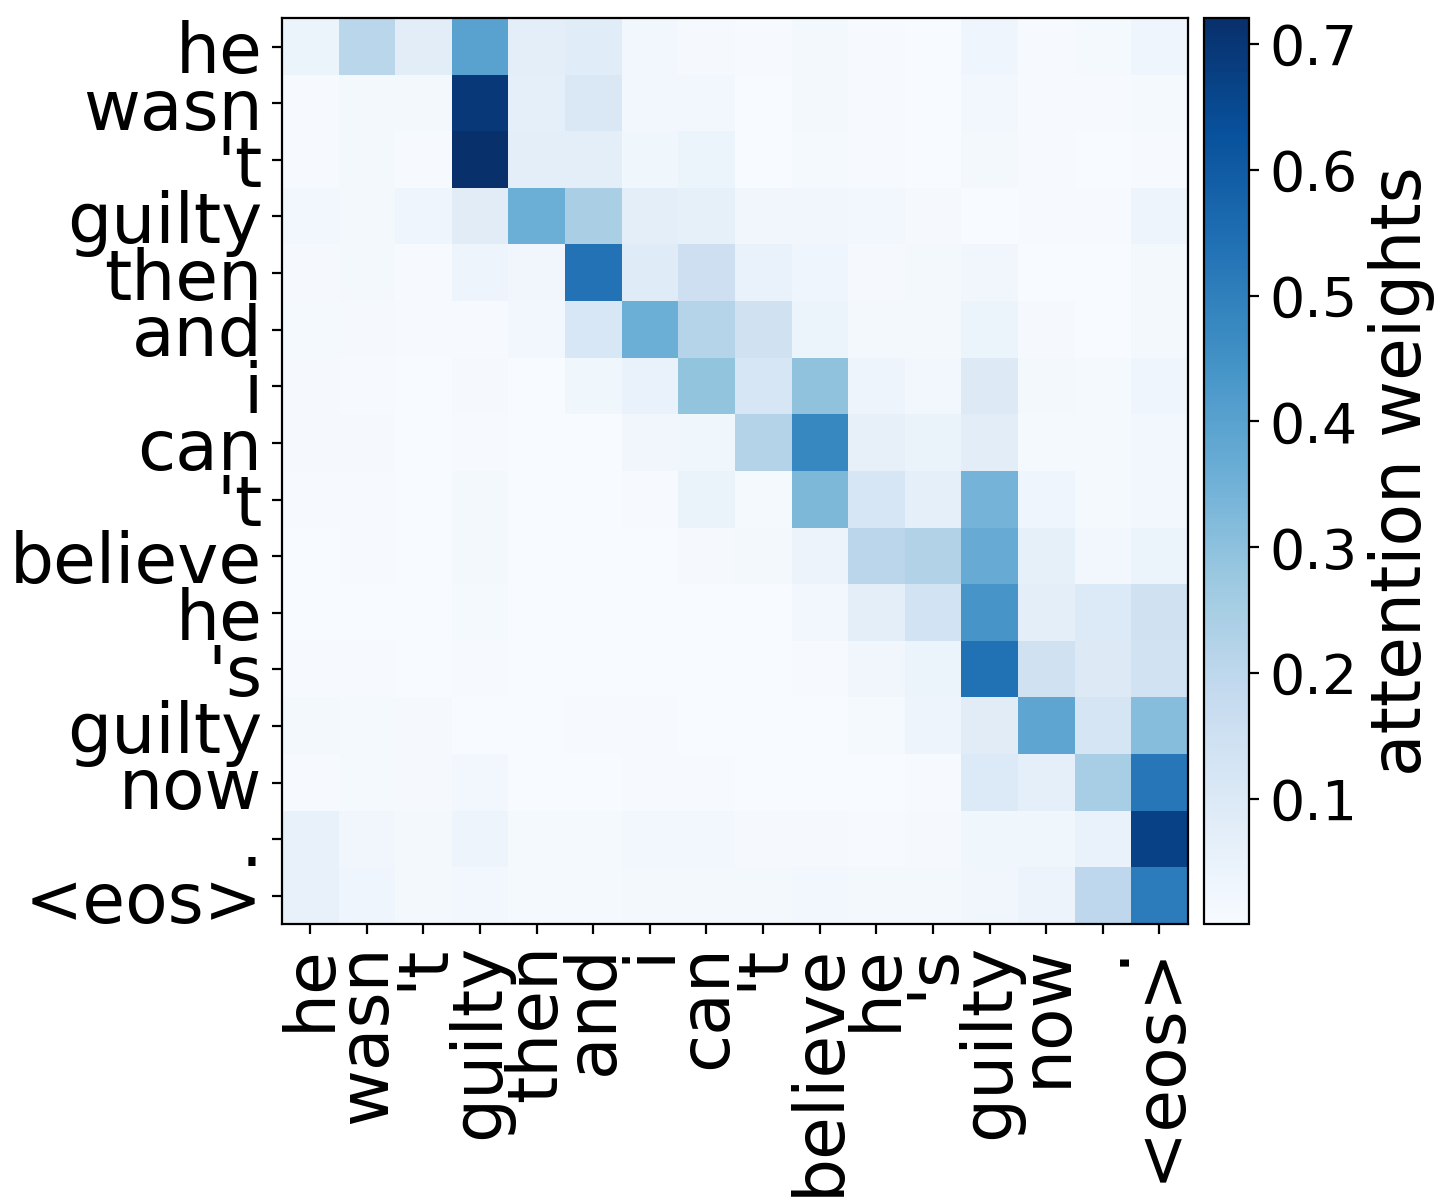
\includegraphics[height=0.50\textheight]{slides/img/04-transformers/voita2019-attention-weights.png}
\end{center}

\vspace{2pt}

\textbf{Exemplo:} self-attention no encoder de um modelo de tradução. A diagonal predominante mostra que cada token atende sobretudo a si mesmo e aos vizinhos.

\vspace{2pt}
\centering
\footnotesize Figura de Voita et al., 2019. \textit{Analyzing multi-head self-attention.}

\end{frame}

% ============================================================

\begin{frame}{Cabeças Especializadas}

Pesquisas (Voita et al., 2019; entre outros) mostram que algumas \textbf{attention heads} se especializam em fenômenos linguísticos conhecidos.

\vspace{6pt}

\begin{block}{Exemplos de especialização observada}
\begin{itemize}
    \item \textbf{Posicional:} a cabeça atende sempre ao token na mesma posição relativa
    \item \textbf{Concordância verbo-sujeito:} liga formas conjugadas ao seu sujeito
    \item \textbf{Objeto-verbo:} liga objetos diretos ao verbo correspondente
    \item \textbf{Palavras raras:} cabeças que ``buscam'' tokens raros para resolver ambiguidade
\end{itemize}
\end{block}

\vspace{6pt}

\begin{exampleblock}{Conclusão}
As cabeças aprendem \textbf{papéis distintos}. Algumas podem ser podadas com perda mínima, sugerindo redundância controlável.
\end{exampleblock}

\end{frame}

% ============================================================
\section*{Referências e Leituras}
% ============================================================

\begin{frame}{Leituras Recomendadas}
    \leiturasize
    \begin{itemize}
        \item Kazemnejad, A. \textit{Transformer Architecture: The Positional Encoding}. \texttt{\footnotesize kazemnejad.com/blog/transformer\_architecture\_positional\_encoding/}
        \item Alammar, J. \textit{The Illustrated Transformer}. \texttt{\footnotesize jalammar.github.io/illustrated-transformer/}
        \item Voita, L. \textit{Sequence to Sequence (seq2seq) and Attention}, NLP Course For You. \texttt{\footnotesize lena-voita.github.io/nlp\_course/seq2seq\_and\_attention.html}. O diagrama do cálculo da self-attention desta aula foi inspirado nas visualizações desse post.
    \end{itemize}
\end{frame}

\begin{frame}{Referências}

\footnotesize

\textbf{Artigos principais:}
\begin{itemize}
    \item Vaswani, A. et al.\ (2017). Attention is All You Need. \textit{Advances in Neural Information Processing Systems}, v.\ 30.
    \item Bahdanau, D., Cho, K., \& Bengio, Y. (2014). Neural Machine Translation by Jointly Learning to Align and Translate. \textit{arXiv:1409.0473}.
    \item Luong, M.-T., Pham, H., \& Manning, C. D. (2015). Effective Approaches to Attention-based Neural Machine Translation. \textit{arXiv:1508.04025}.
\end{itemize}

\vspace{4pt}

\textbf{Componentes:}
\begin{itemize}
    \item He, K., Zhang, X., Ren, S., \& Sun, J. (2016). Deep Residual Learning for Image Recognition. \textit{CVPR}.
    \item Ba, J. L., Kiros, J. R., \& Hinton, G. E. (2016). Layer Normalization. \textit{arXiv:1607.06450}.
\end{itemize}

\vspace{4pt}

\textbf{Análise e interpretabilidade:}
\begin{itemize}
    \item Voita, E., Talbot, D., Moiseev, F., Sennrich, R., \& Titov, I. (2019). Analyzing Multi-Head Self-Attention: Specialized Heads Do the Heavy Lifting, the Rest Can Be Pruned. \textit{arXiv:1905.09418}.
\end{itemize}

\end{frame}

\end{document}
